\documentclass[a4paper]{article}
\usepackage{fullpage}
\usepackage[utf8]{inputenc}
\usepackage{mathtools}
\usepackage[defaultsans]{comfortaa}
\usepackage[T1]{fontenc}
\usepackage{float}
\usepackage{hyperref}
\usepackage{multicol}
\usepackage{wrapfig}
\usepackage{subcaption}

\title{\Large{\textbf{Relatório Final: Análise de Longarina em Estrutura de Asa para o Avião de Pesquisa Phoenix P2}}}
\author{Gustavo Mancuso Bolson}

\begin{document}

\maketitle

\section{Introdução}

Este relatório é o seguinte da \textit{Proposta de Projeto} após as análises e decisões principais da estrutura das asas do projeto Phoenix P2, o qual \textit{in memoriae} é parte integrante de um esforço multidisciplinar de capacitar e desenvolver conhecimentos que permitam uma maior experiência na área de atuação aeroespacial durante a graduação, através do design, construção, realização de ensaios e voos-teste de um avião não-tripulado de características facilmente modificáveis.

Foi realizada uma série de simulações com dois métodos principais: utilizando uma simulação de barra como o estudado na disciplina com esforços mais precisos e um com diferenças finitas que permite maior controle sobre as características da barra que tem a vantagem de oferecer valores confiáveis de limites de escoamento dos materiais testados mas exige algumas simplificações no cálculo dos esforços. Desta forma podemos ter uma discussão informada sobre qual a escolha mais adequada de material e melhoras para o design proposto inicialmente dentro das escalas fornecidas pelos requisitos, que também são avaliados por conformidade neste relatório.

\section{Determinação de Esforços Aerodinâmicos}

Para determinar os esforços aerodinâmicos atuantes nas asas durante operação que não excede os limites mínimos do envelope de voo esperado, uma série de condições para a carga podem ser modeladas: 

A primeira e mais relevante é que a pressão em toda a superfície da asa é contínua e suavemente variável, o que elimina a validade da análise para uma condição de estol com fluxo altamente turbilhonar e caótico. A decisão é justificada pelas cargas envolvidas serem menores do que as esperadas pela própria natureza deste estado de operação, que envolve uma combinação de ângulo de ataque $\alpha$ elevado combinado com uma baixa velocidade verdadeira do ar. Em conjunto a isso e para evitar prolongações burocráticas acordo com as regras de operação de aeromodelos da Agência Nacional de Aviação Civil (ANAC), a variação de densidade do ar em função à altura máxima de 400 pés AGL \cite{anacdrones} não será considerável o suficiente para afetar a análise, que foi feita utilizando uma temperatura aproximada de 20°C a nível do mar.

A segunda é de que as forças que atuam em cada contato com as nervuras mantém-se constantes com relação às coordenadas locais independentemente de deflexão da longarina. Esta condição é válida pois o perfil de pressão local em um corte a uma distância fixa do engaste da asa é determinado apenas pela forma do aerofólio, seu ângulo de ataque $\alpha$ e o número de Reynolds $R_e$ do fluxo. De acordo com a área planiforme retangular das asas, a razão entre envergadura e comprimento de corda de 10, e a desconsideração dos efeitos aerodinâmicos do engaste de ajuste e corpo da aeronave, podemos utilizar a seguinte equação para aproximar a um coeficiente de distribuição de pressão $\Gamma(y)$ da proporção de distância do engaste x. os valores de $a$ e $k$ são dependentes da razão entre corda e envergadura da asa. Se tomamos o valor de $k=1$ (indicando que os valores de y são em semi-envergadura percorrida normalizada), podemos modelar através de um \textit{fit} \cite{WPIpaper} e então determinar o valor de $a\approx 7.6$.

\vspace{0.5cm}

\begin{equation}
    \Gamma(y) = 1-\left(e^{-a\left(y+k\right)}+e^{a\left(y-k\right)}\right)
\end{equation}

\vspace{0.5cm}

Finalmente, para calcular o perfil de pressões em uma seção de aerofólio, foi utilizado um software de simulação/banco de dados XFOIL \cite{xfoil}. Foram escolhidos 3 estados segundo o envelope de voo mínimo, os quais são apresentados a seguir com suas condições de contorno e os resultados de distribuições de pressão que são condensados em forças pontuais para modelagem dos esforços na longarina. Os estados são escolhidos segundo os diagramas polares do aerofólio escolhido (NACA 23015) nos regimes esperados \cite{aftools}.

\begin{figure}[H]
    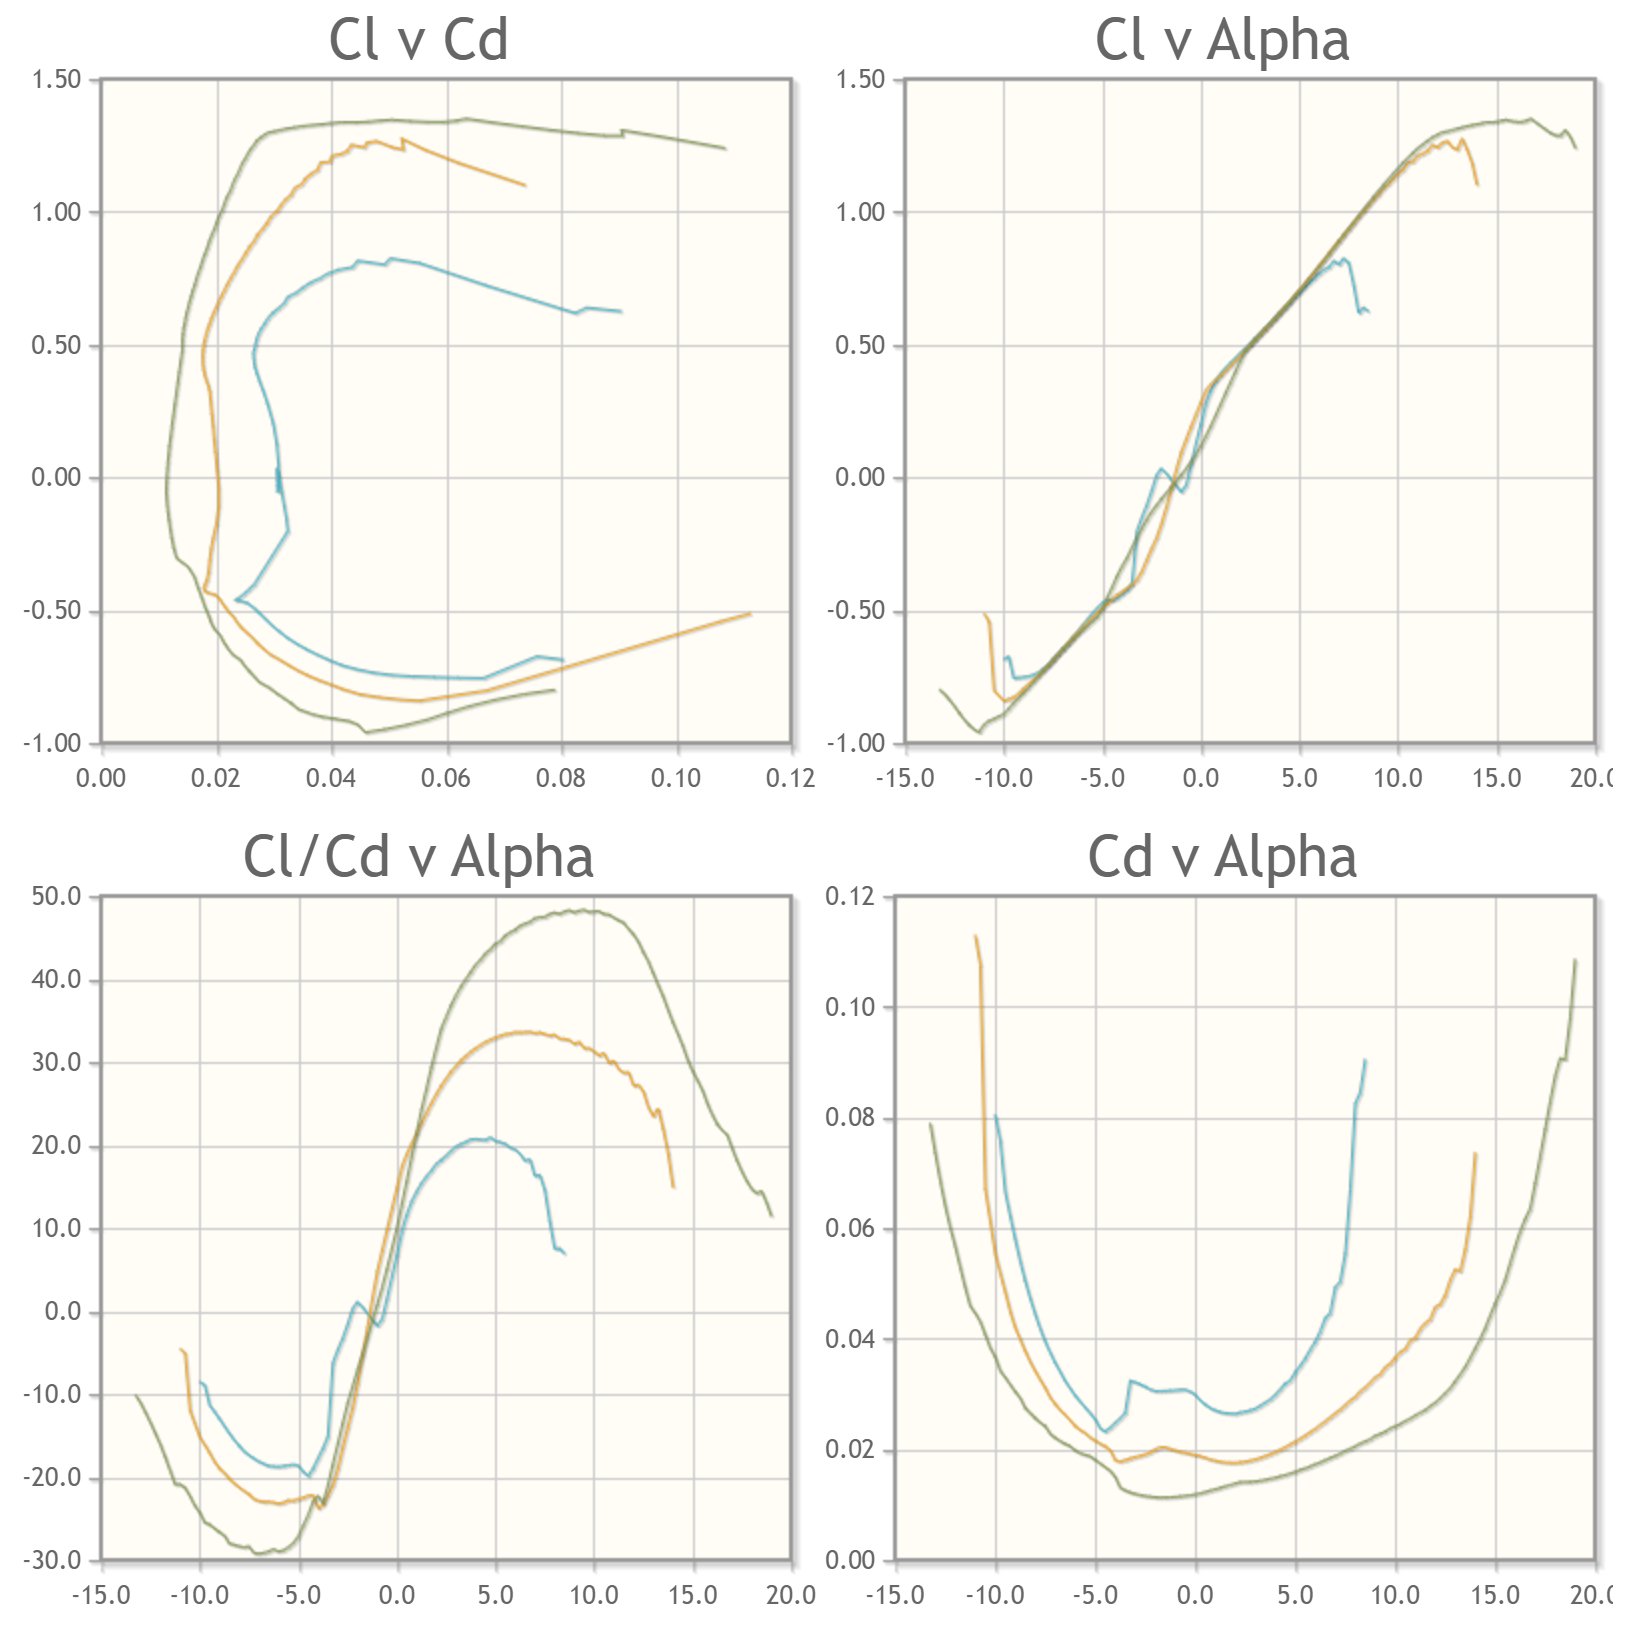
\includegraphics[width=\textwidth]{Polars.png}
\end{figure}

A seguir apresentamos 4 estados de operação esperados do aerofólio, incluindo em uma velocidade média esperada para voos iniciais e pré-pousos e outras 3 nas velocidades máximas esperadas variando apenas o ângulo de ataque. Como o terceiro estado (análogo a uma curva coordenada com a maior aceleração centrípeta à maior velocidade esperada) apresenta a maior carga à qual as asas estarão submetidas, esta será a considerada para a análise de esforços. É importante lembrar que qualquer ângulo maior do que 15° a um $R_e=2\times10^5$ resulta em condição de estol, o que reduz a carga na asas.

\begin{figure}[H]
    \begin{subfigure}[b]{0.48\textwidth}
      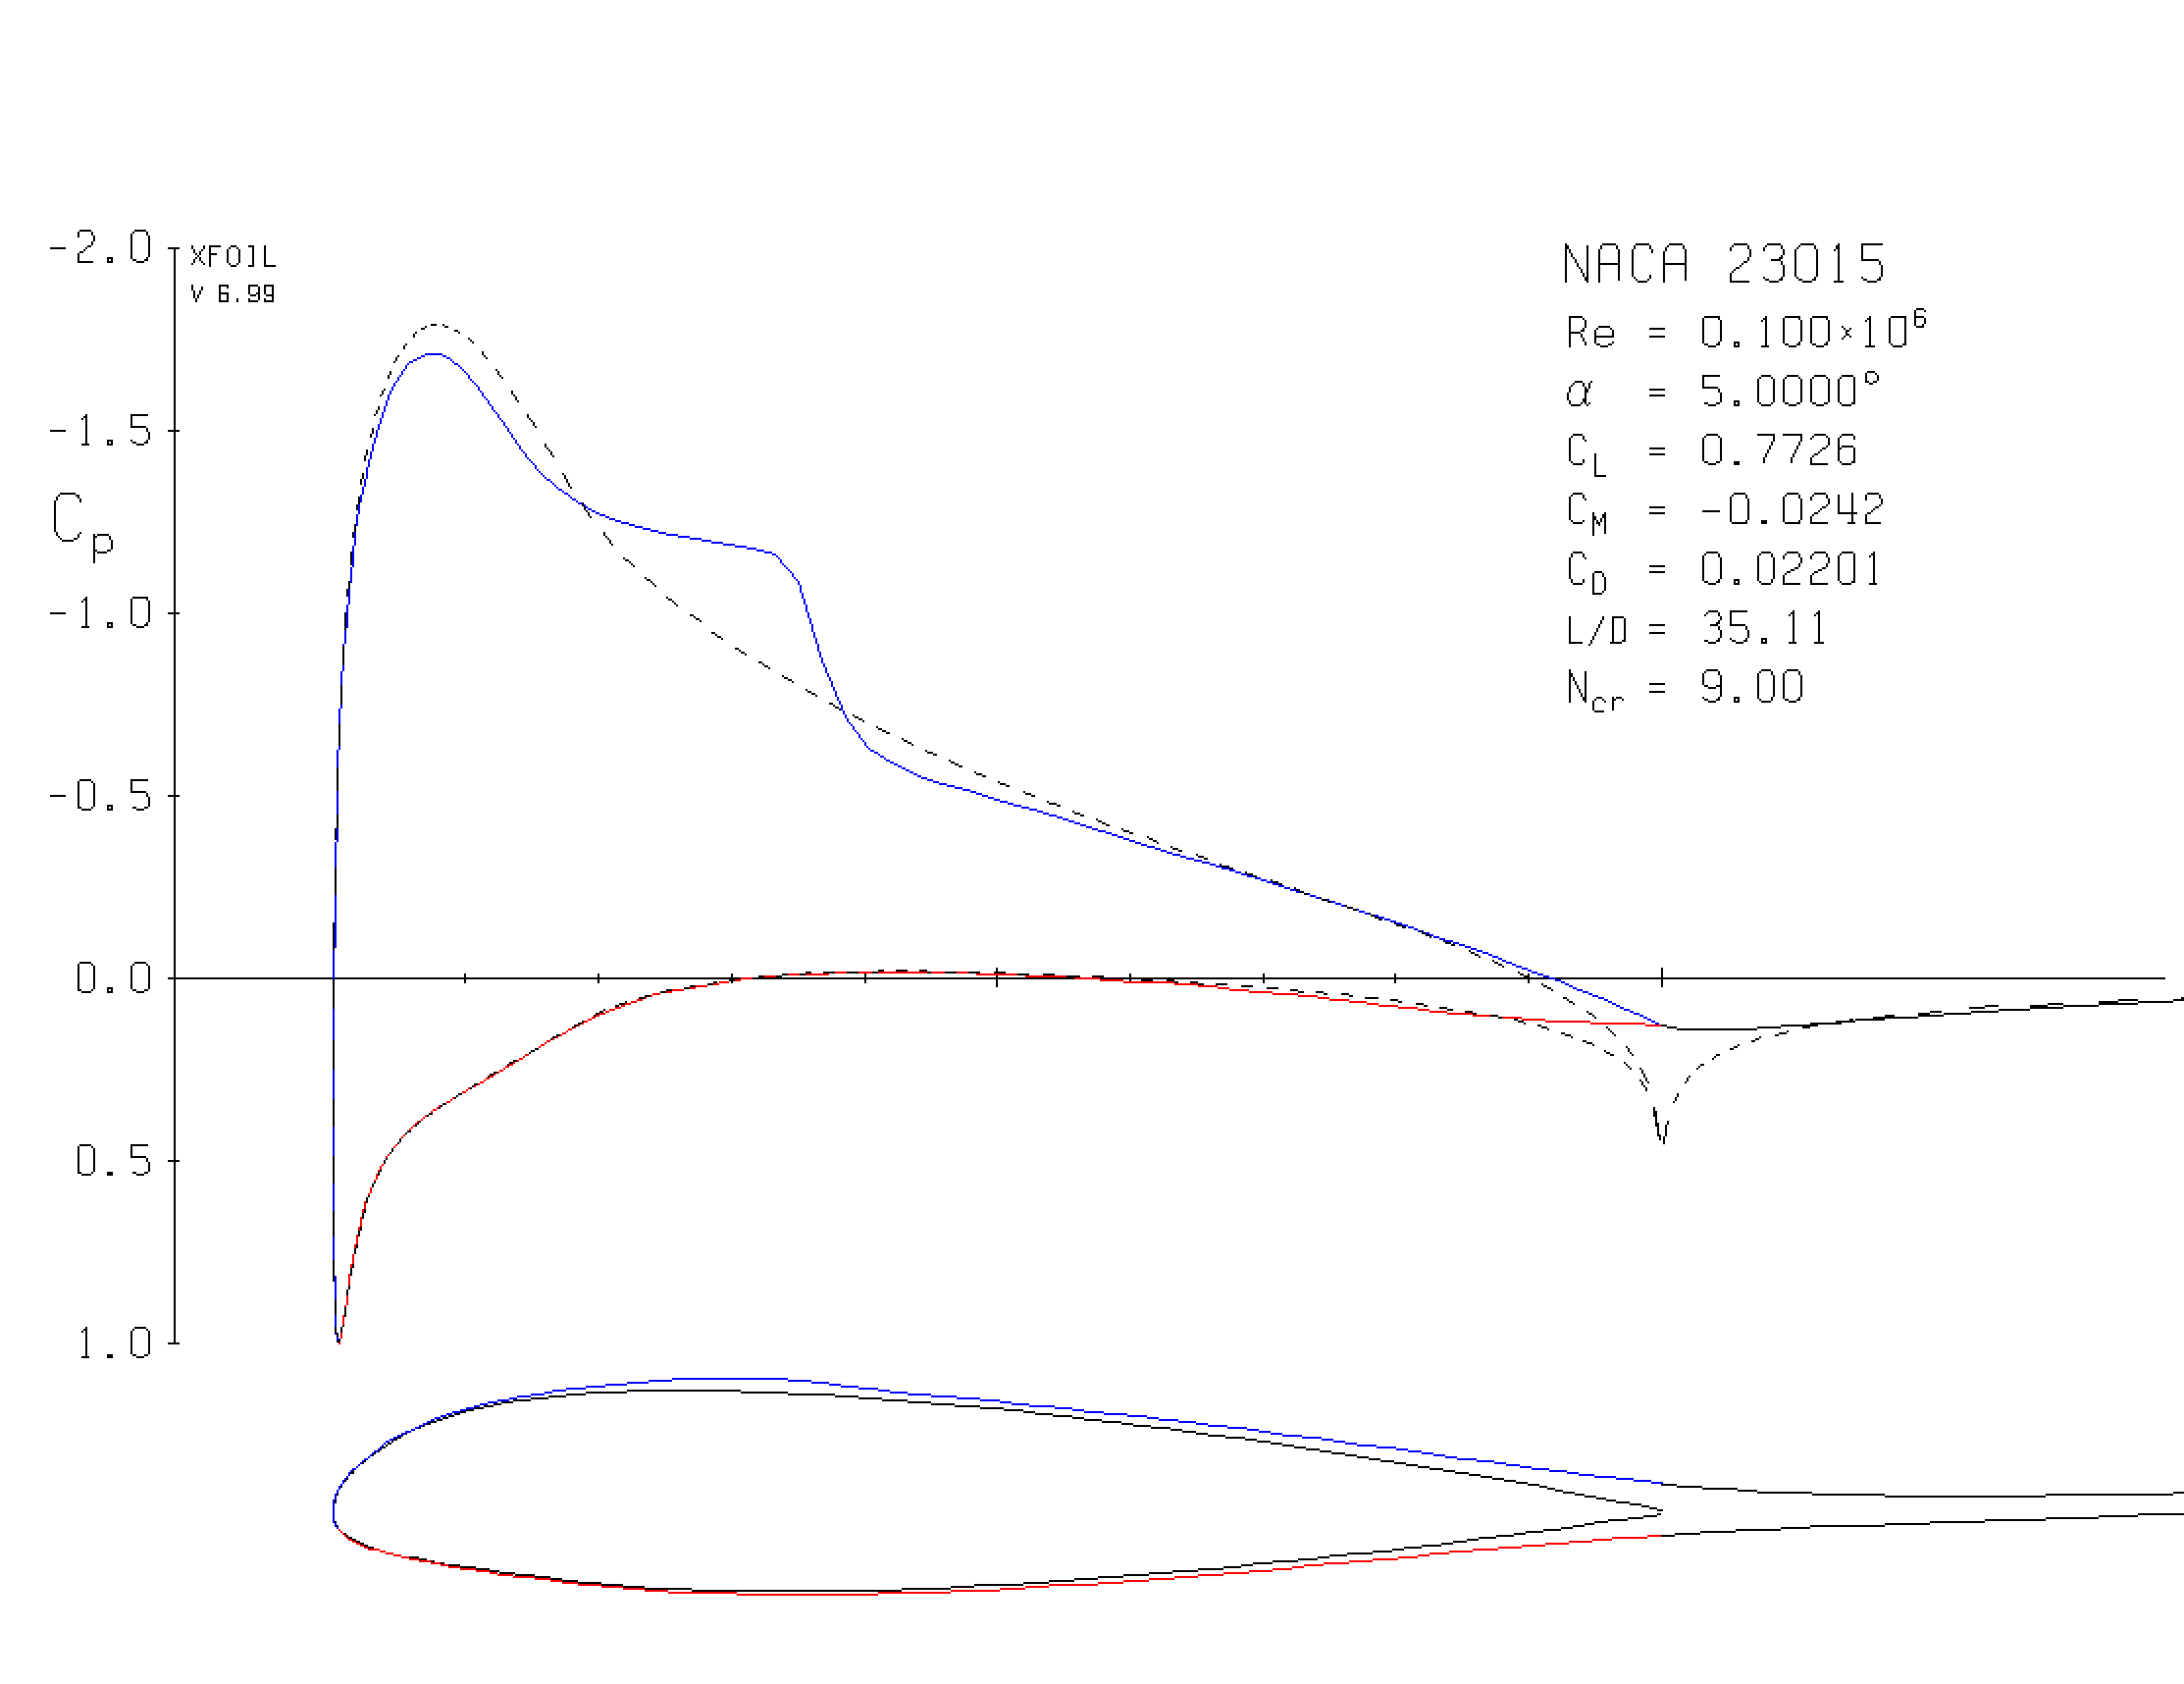
\includegraphics[width=\textwidth]{Re1e5_a5.png}
      \caption*{Operação Normal: $\alpha$ = 5° a 8m/s}
    \end{subfigure}
    %
    \begin{subfigure}[b]{0.48\textwidth}
      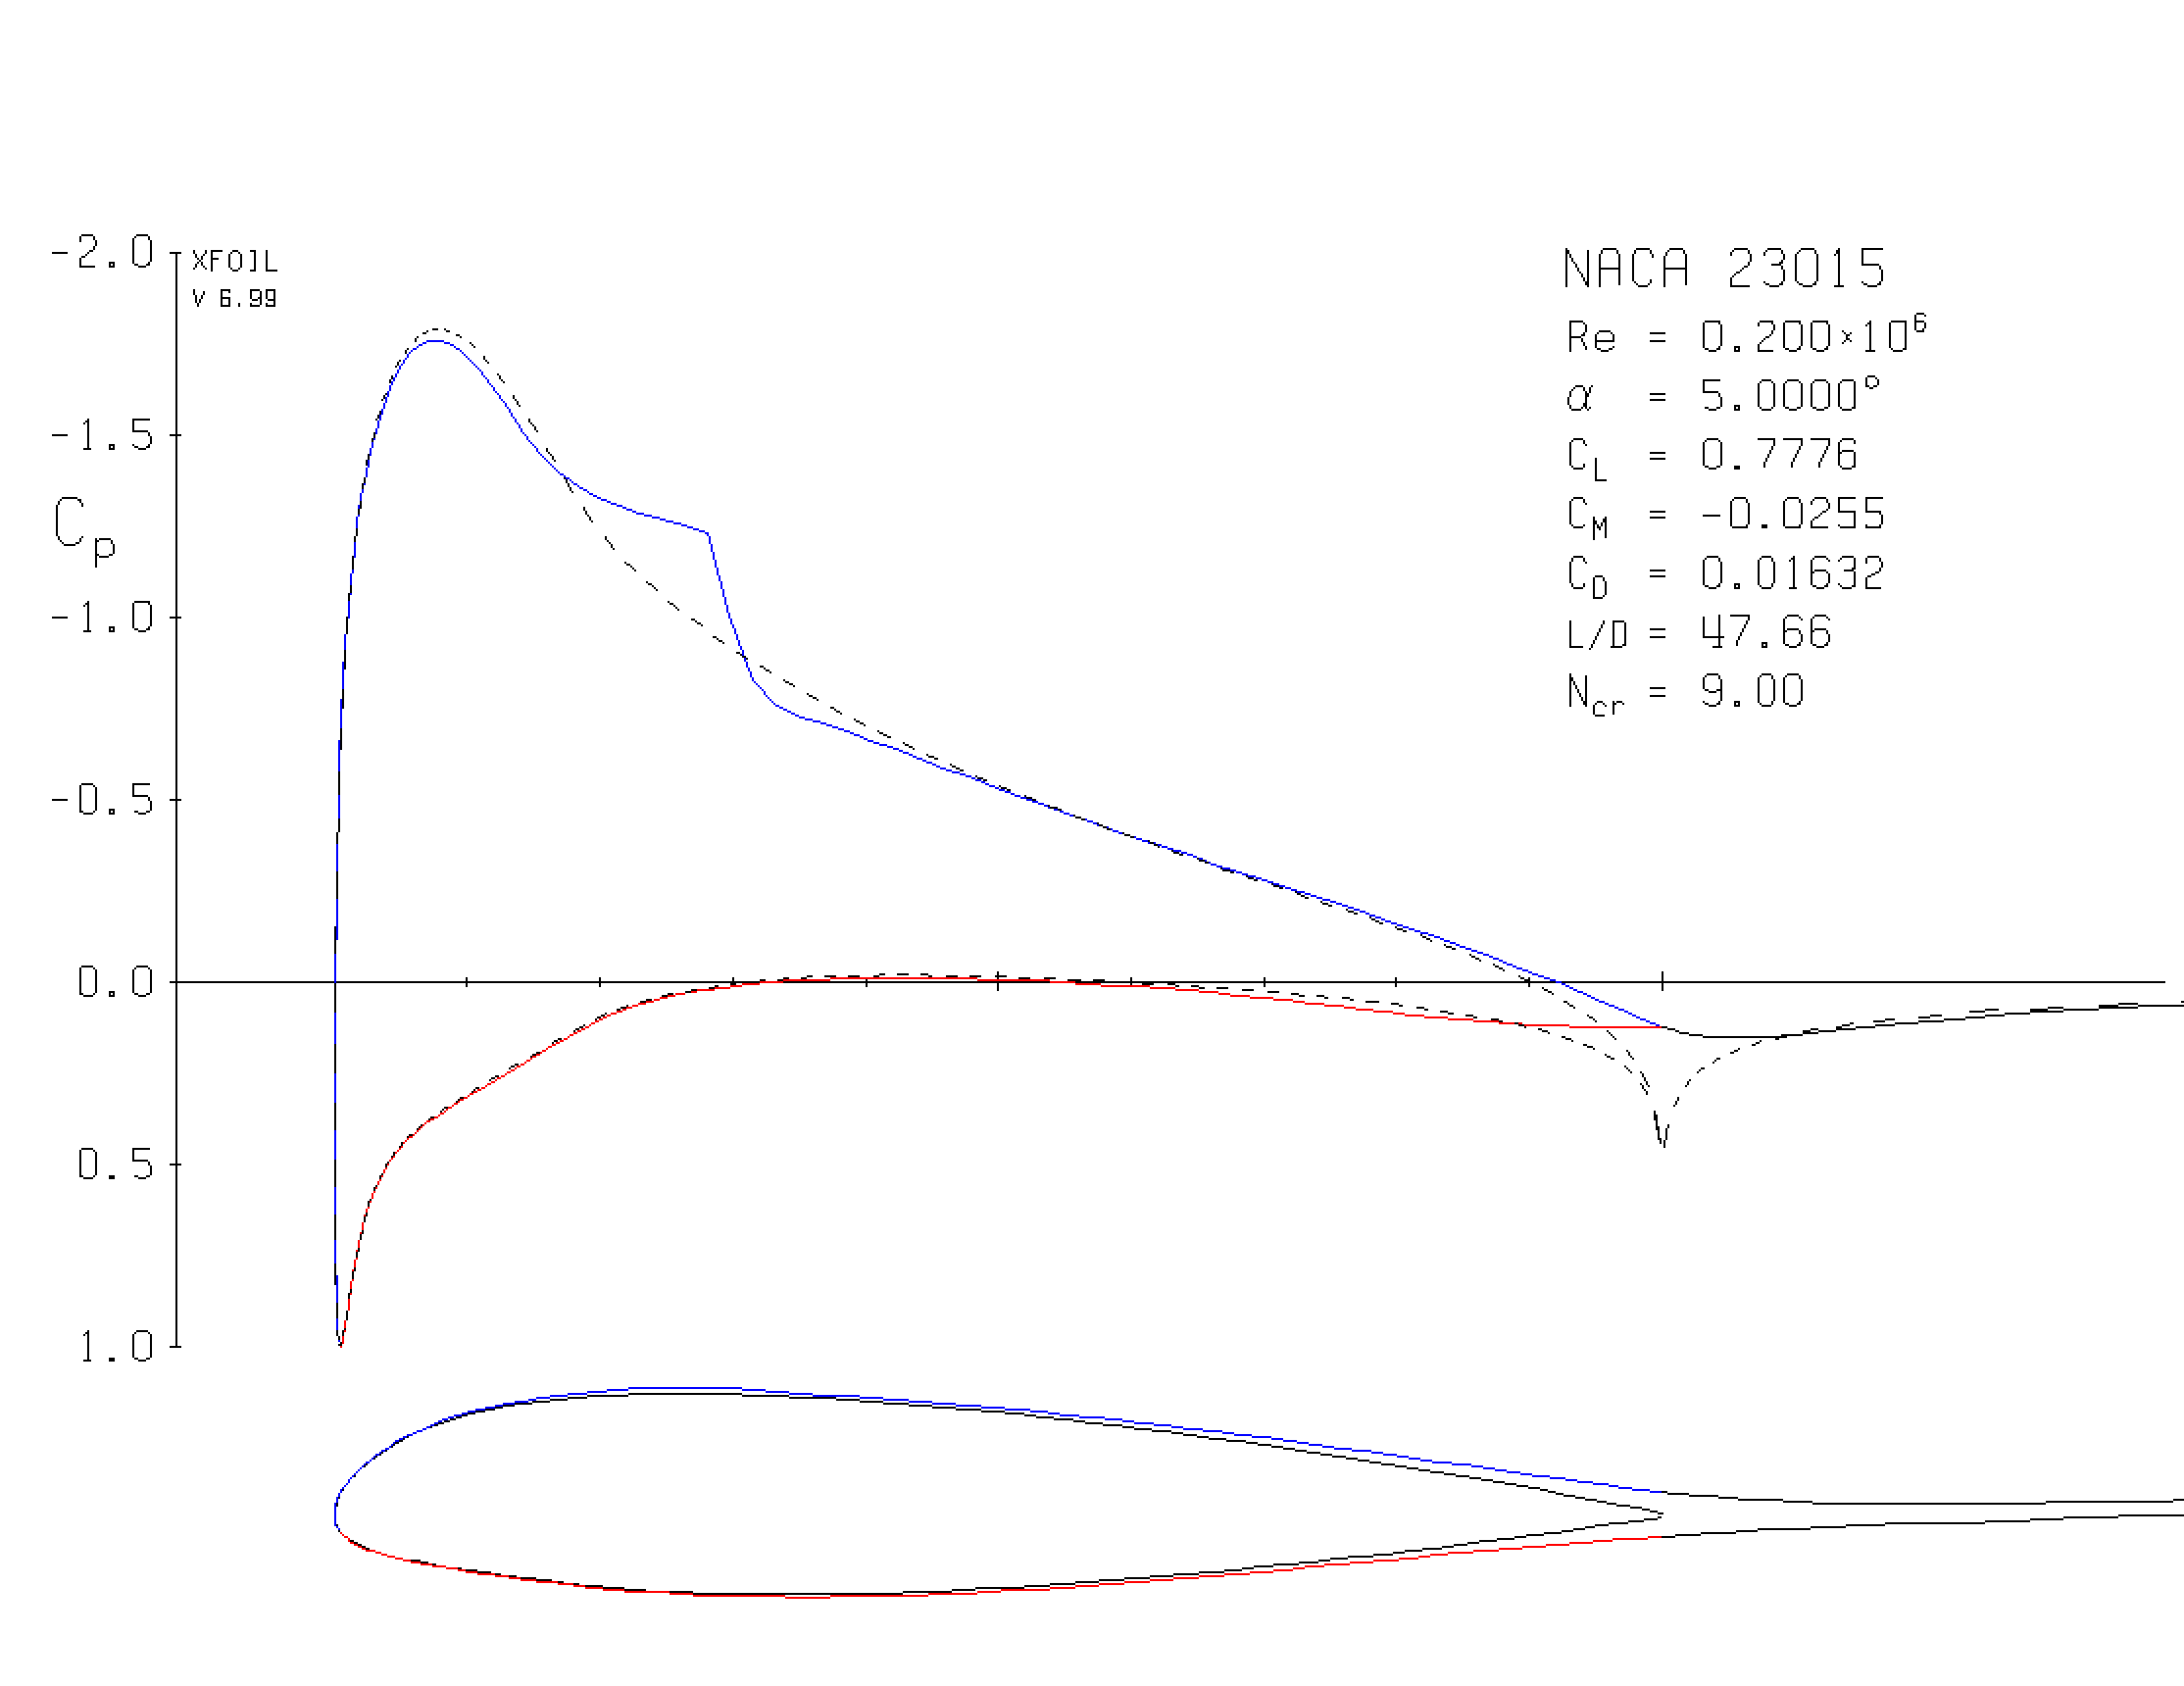
\includegraphics[width=\textwidth]{Re2e5_a5.png}
      \caption*{Max. Velocidade: $\alpha$ = 5° a 15m/s}
    \end{subfigure}
\end{figure}

\begin{figure}[H]
    \begin{subfigure}[b]{0.48\textwidth}
      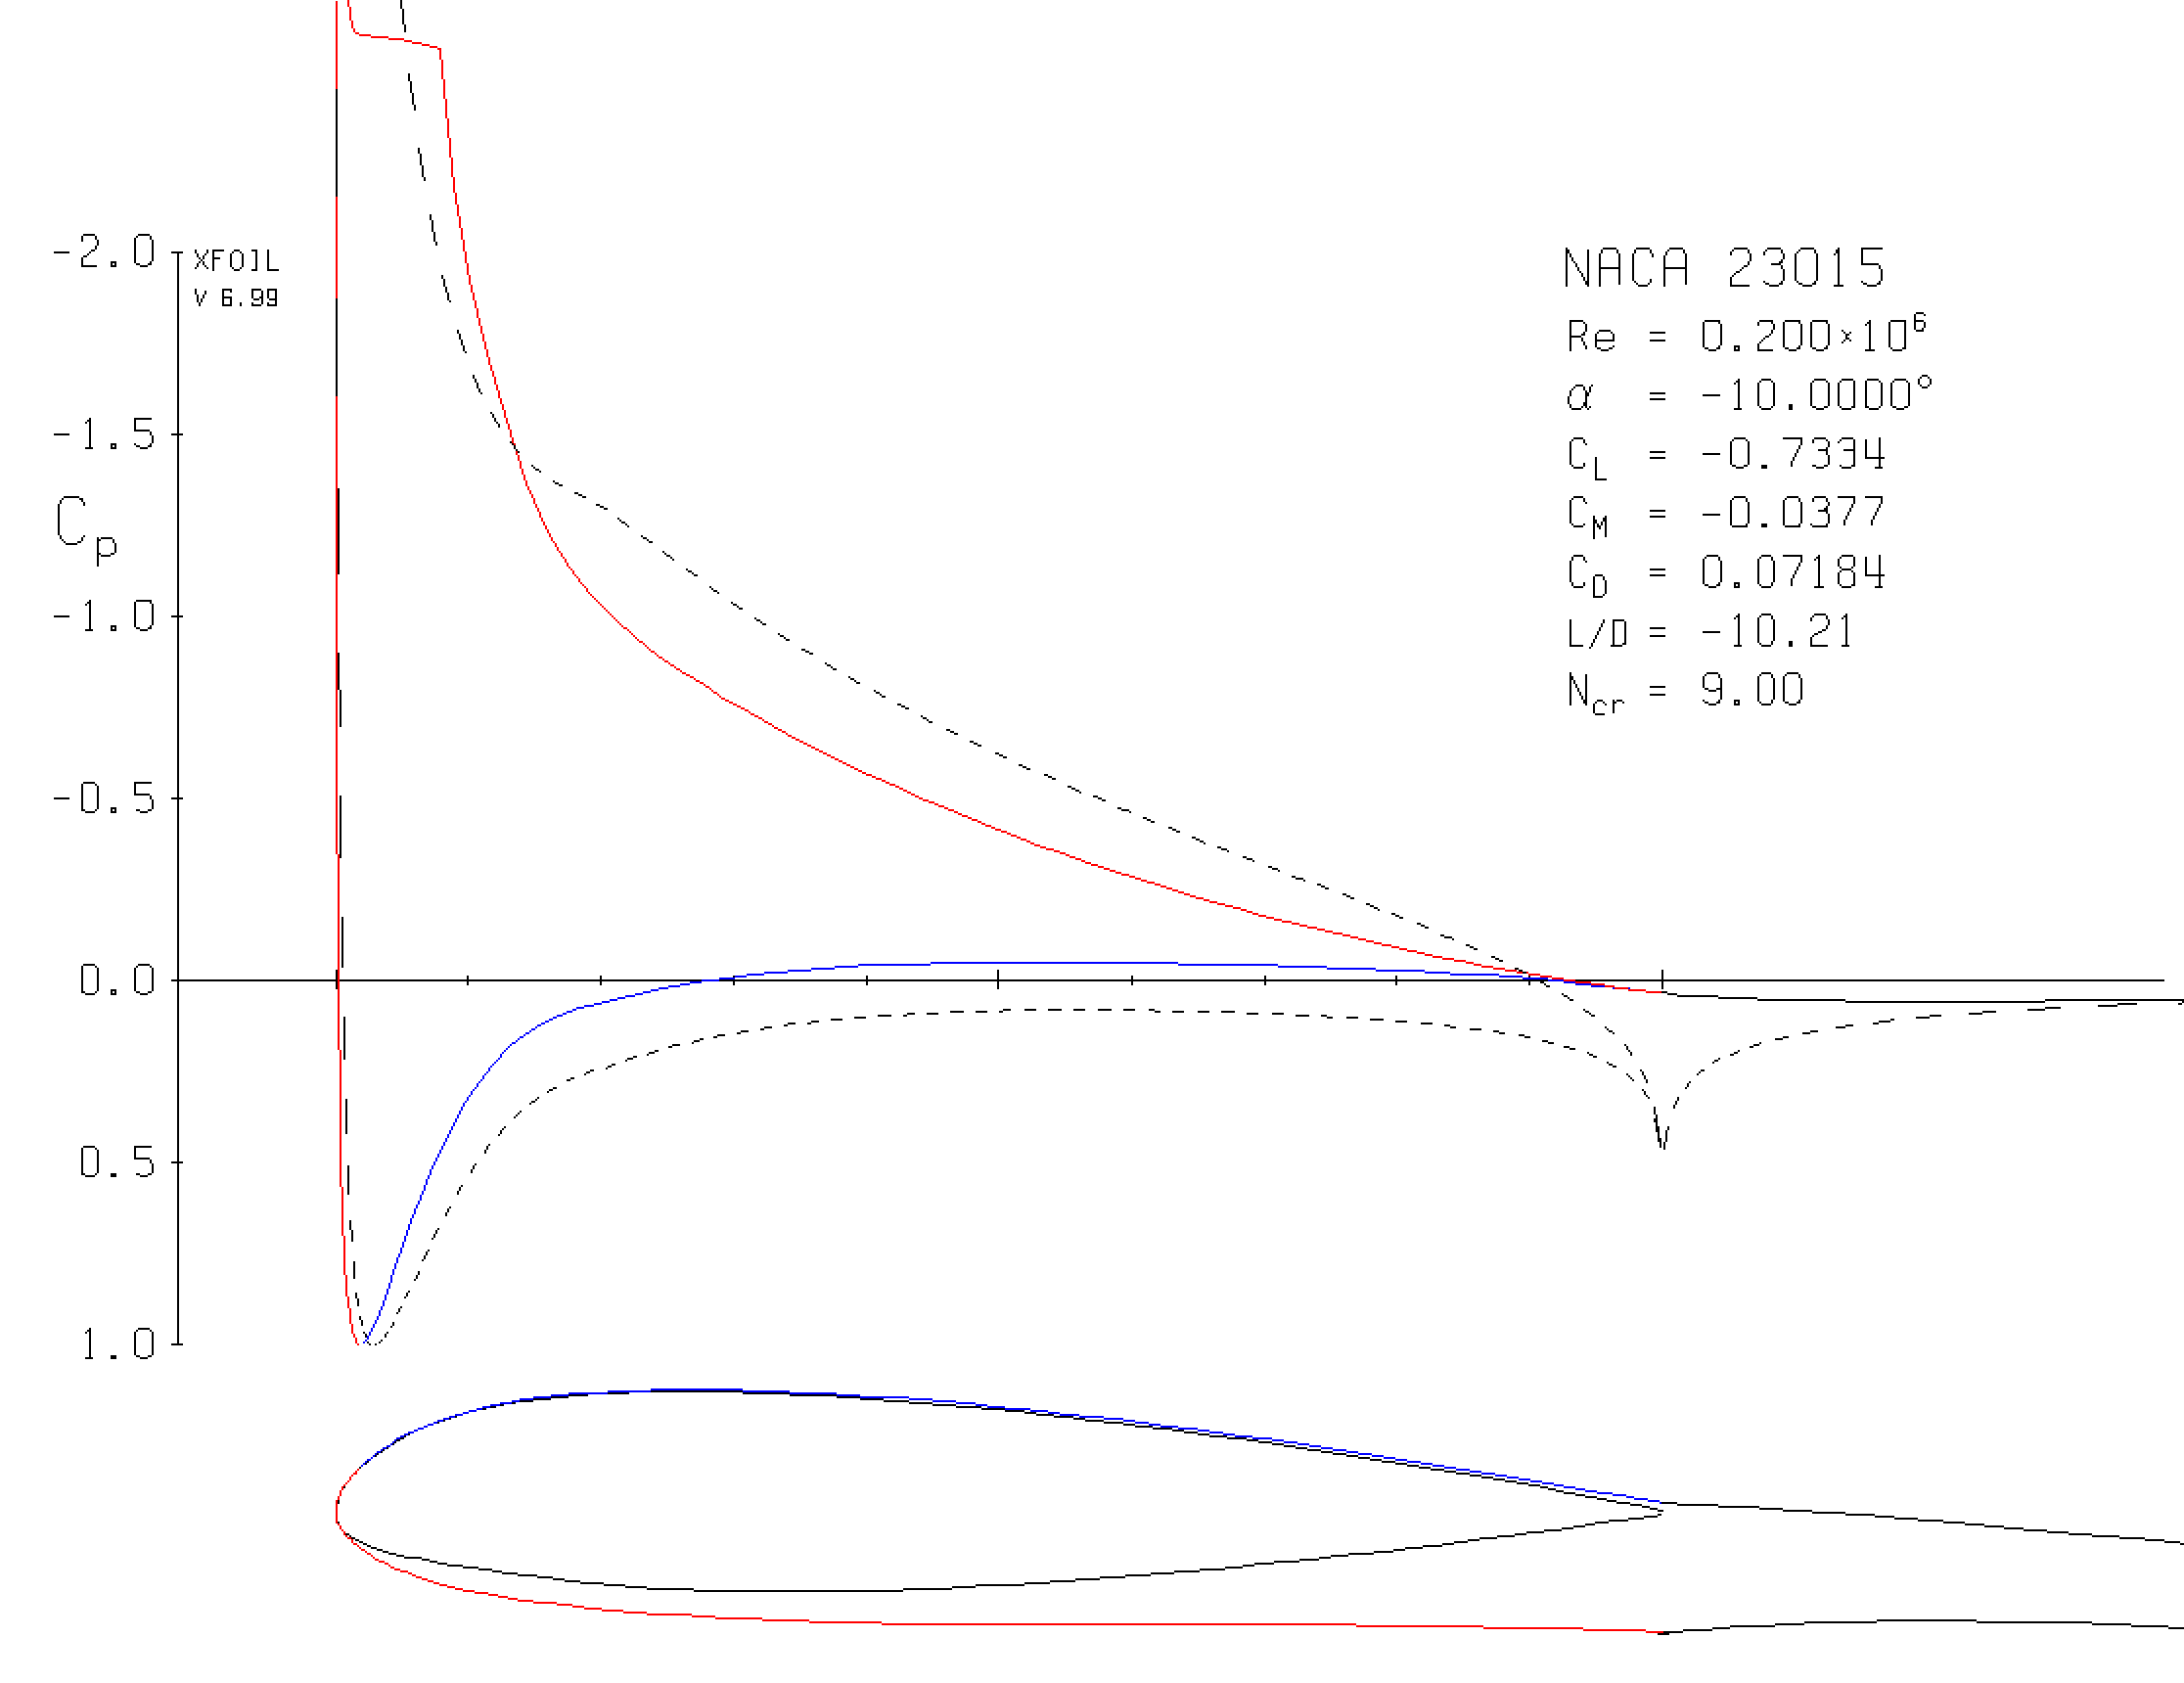
\includegraphics[width=\textwidth]{Re2e5_a-10.png}
      \caption*{Max. Velocidade: $\alpha$ = -10° a 15m/s}
    \end{subfigure}
    %
    \begin{subfigure}[b]{0.48\textwidth}
      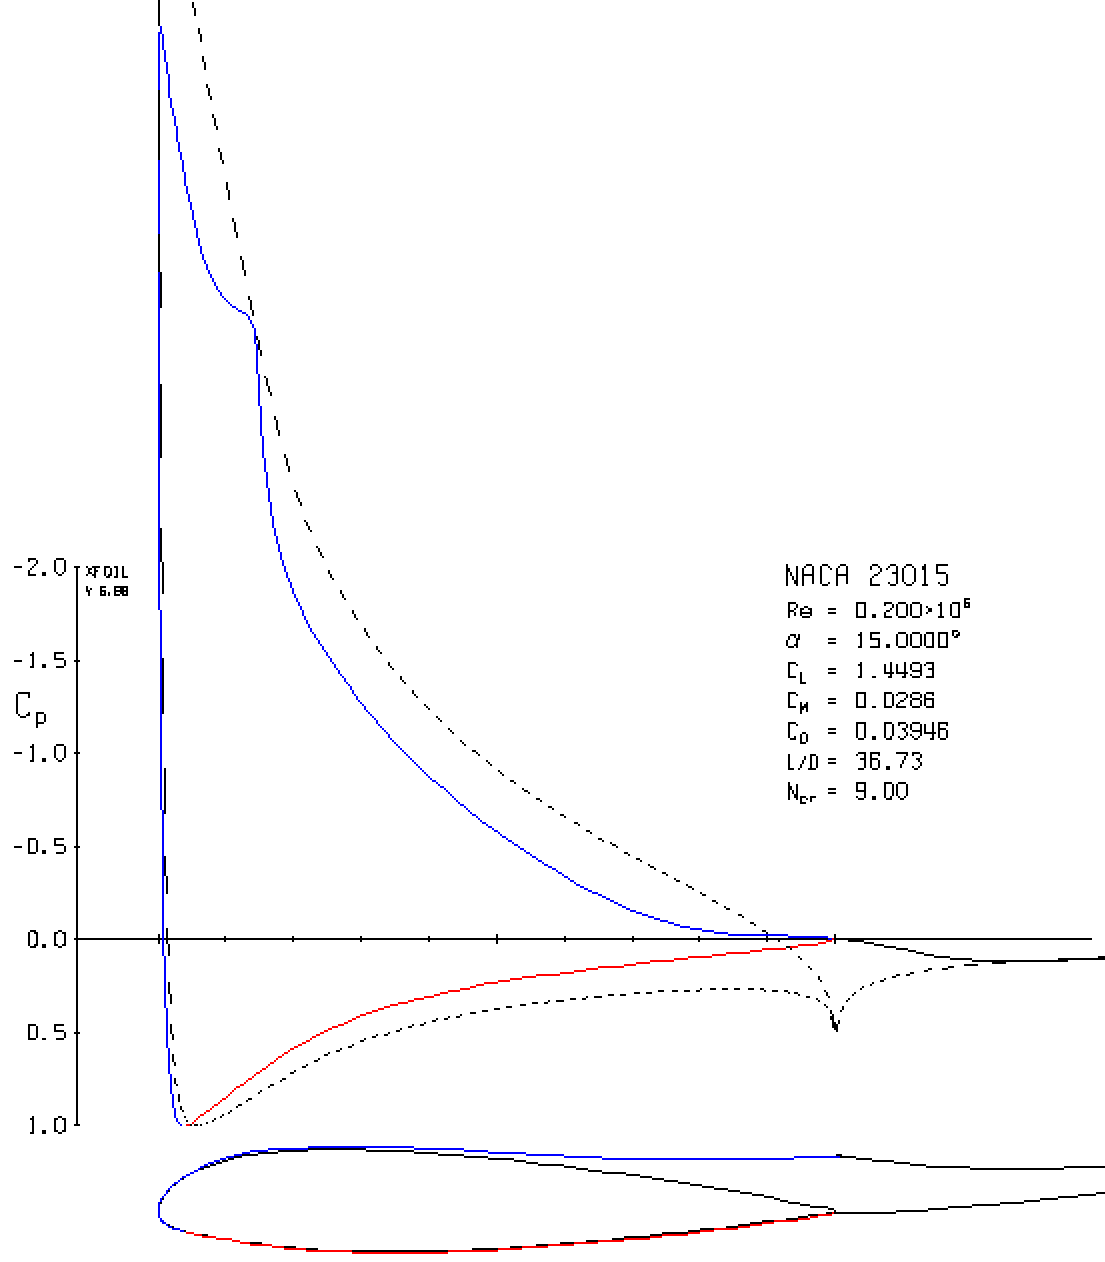
\includegraphics[width=\textwidth]{Re2e5_a15.png}
      \caption*{Max. Velocidade: $\alpha$ = 15° a 15m/s}
    \end{subfigure}
\end{figure}


Por fim, podemos tomar os coeficientes adquiridos para calcular quais são as forças de sustentação e arrasto segundo as equações (2) e (3) respectivamente. Os pontos de aplicação da força $L$ e, por consequência, torques envolvidos em cada seção de área é calculada por um \textit{fit} de spline dos diagramas acima, e o perfil é modelado linearmente em coeficiente de $\Gamma(y)$. As equações consideram o centro de coordenadas como sendo a linha de ataque do aerofólio. As medidas são considerando envergadura e corda normalizadas para 1, e são aplicadas para cada nervura. Os termos adicionais são derivados da teoria apresentada por Anderson (2017) \cite{anderson}. Todos as formulas utilizam unidades do sistema internacional.

\vspace{0.5cm}

\begin{minipage}{.47\linewidth}
    \begin{equation}
        L_n = C_L \frac{1}{2} \rho V^2 l \int_{y_{n-1}}^{y_{n+1}} \frac{\Gamma(y)}{2} dy
    \end{equation}
    \begin{equation}
        D_n = C_D \frac{1}{2} \rho V^2 l \int_{y_{n-1}}^{y_{n+1}} \frac{\Gamma(y)}{2} dy + D_0
    \end{equation}
\end{minipage}
\begin{minipage}{.47\linewidth}
    \begin{equation}
        M_x = L (y_L) + C_L \frac{1}{2} \rho V^2 l (1 - \int_{y_{n-1}}^{y_{n+1}} \frac{\Gamma(y)}{2} dy) = 0
    \end{equation}
    \begin{equation}
        M_y = L (x_L - 0.3)
    \end{equation}
    \begin{equation}
        M_z = 0
    \end{equation}
\end{minipage}

\vspace{0.5cm}

\section{Análise de Esforços na Longarina}

Para a execução dos cálculos, foi utilizado a ferramenta de simulação estática do SolidWorks com 10 segmentos como os especificados na \textit{Proposta de Projeto}. Para motivo desta primeira análise, a geometria da seção reta pode ser desconsiderada quando tratamos dos esforços. Em cada junção da barra foi aplicado um par de forças linearmente independentes e um momento torsor, que estão representados na tabela abaixo:

\begin{table}[H]
    \begin{tabular}{llllllllllll}
    y{[}$m${]}   & 0                          & 0.1                         & 0.2                         & 0.3                         & 0.4                         & 0.5                         & 0.6                         & 0.7                         & 0.8                         & 0.9                        & 1                          \\ \cline{2-12} 
    \multicolumn{1}{l|}{$L$} & \multicolumn{1}{l|}{9.804} & \multicolumn{1}{l|}{19.602} & \multicolumn{1}{l|}{19.579} & \multicolumn{1}{l|}{19.524} & \multicolumn{1}{l|}{19.404} & \multicolumn{1}{l|}{19.147} & \multicolumn{1}{l|}{18.598} & \multicolumn{1}{l|}{17.423} & \multicolumn{1}{l|}{14.911} & \multicolumn{1}{l|}{9.540} & \multicolumn{1}{l|}{2.940} \\ \cline{2-12} 
    \multicolumn{1}{l|}{$D$}     & \multicolumn{1}{l|}{1.482} & \multicolumn{1}{l|}{1.481}  & \multicolumn{1}{l|}{1.481}  & \multicolumn{1}{l|}{1.479}  & \multicolumn{1}{l|}{1.476}  & \multicolumn{1}{l|}{1.469}  & \multicolumn{1}{l|}{1.454}  & \multicolumn{1}{l|}{1.422}  & \multicolumn{1}{l|}{1.354}  & \multicolumn{1}{l|}{1.207} & \multicolumn{1}{l|}{1.028} \\ \cline{2-12} 
    \multicolumn{1}{l|}{$M_y$}     & \multicolumn{1}{l|}{0.686} & \multicolumn{1}{l|}{1.372}  & \multicolumn{1}{l|}{1.370}  & \multicolumn{1}{l|}{1.366}  & \multicolumn{1}{l|}{1.358}  & \multicolumn{1}{l|}{1.340}  & \multicolumn{1}{l|}{1.301}  & \multicolumn{1}{l|}{1.219}  & \multicolumn{1}{l|}{1.043}  & \multicolumn{1}{l|}{0.667} & \multicolumn{1}{l|}{0.205} \\ \cline{2-12} 
    \end{tabular}
\end{table}

Com os valores acima podemos então obter os resultados apresentados abaixo para todos os esforços solicitantes na barra. É interessante observar que a discretização de 11 nervuras ao longa da longarina já permite uma aproximação considerável de uma pressão contínua agindo sobre a barra. É importante notar que o programa usa outra convenção de representação da utilizada na disciplina.

\begin{figure}[H]
    \begin{subfigure}[b]{0.48\textwidth}
      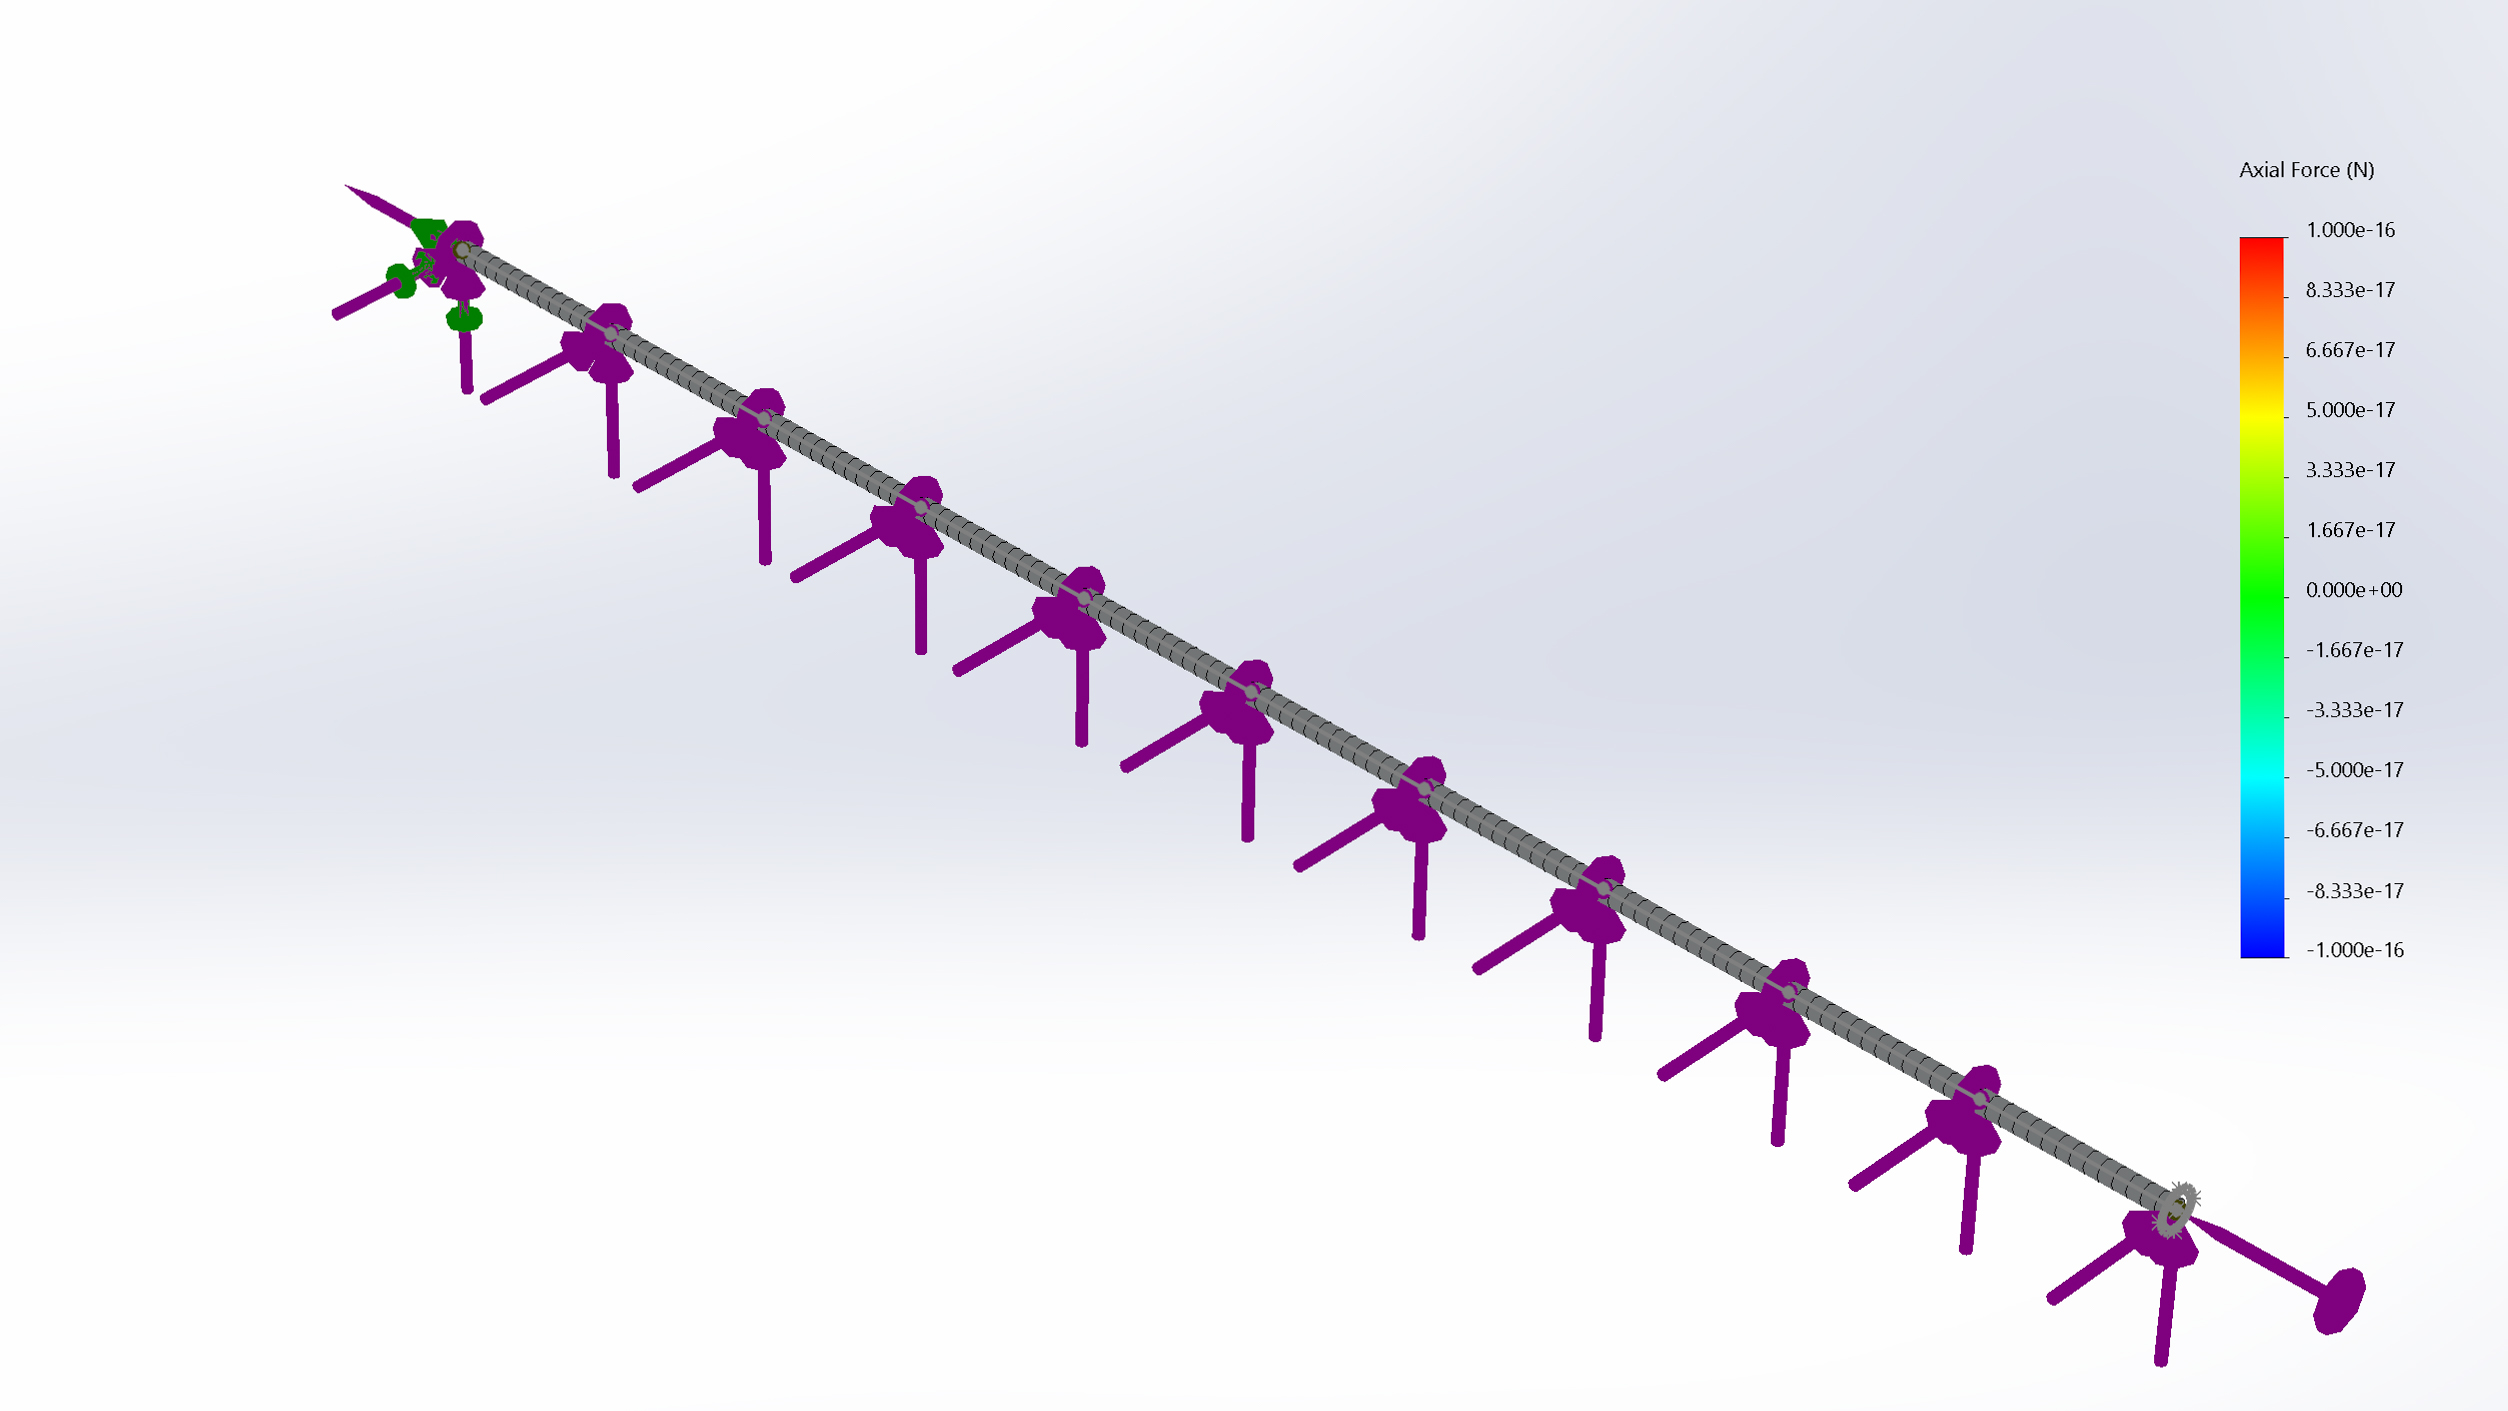
\includegraphics[width=\textwidth]{N.jpg}
      \caption*{Força normal $N(y)$}
    \end{subfigure}
    %
    \begin{subfigure}[b]{0.48\textwidth}
      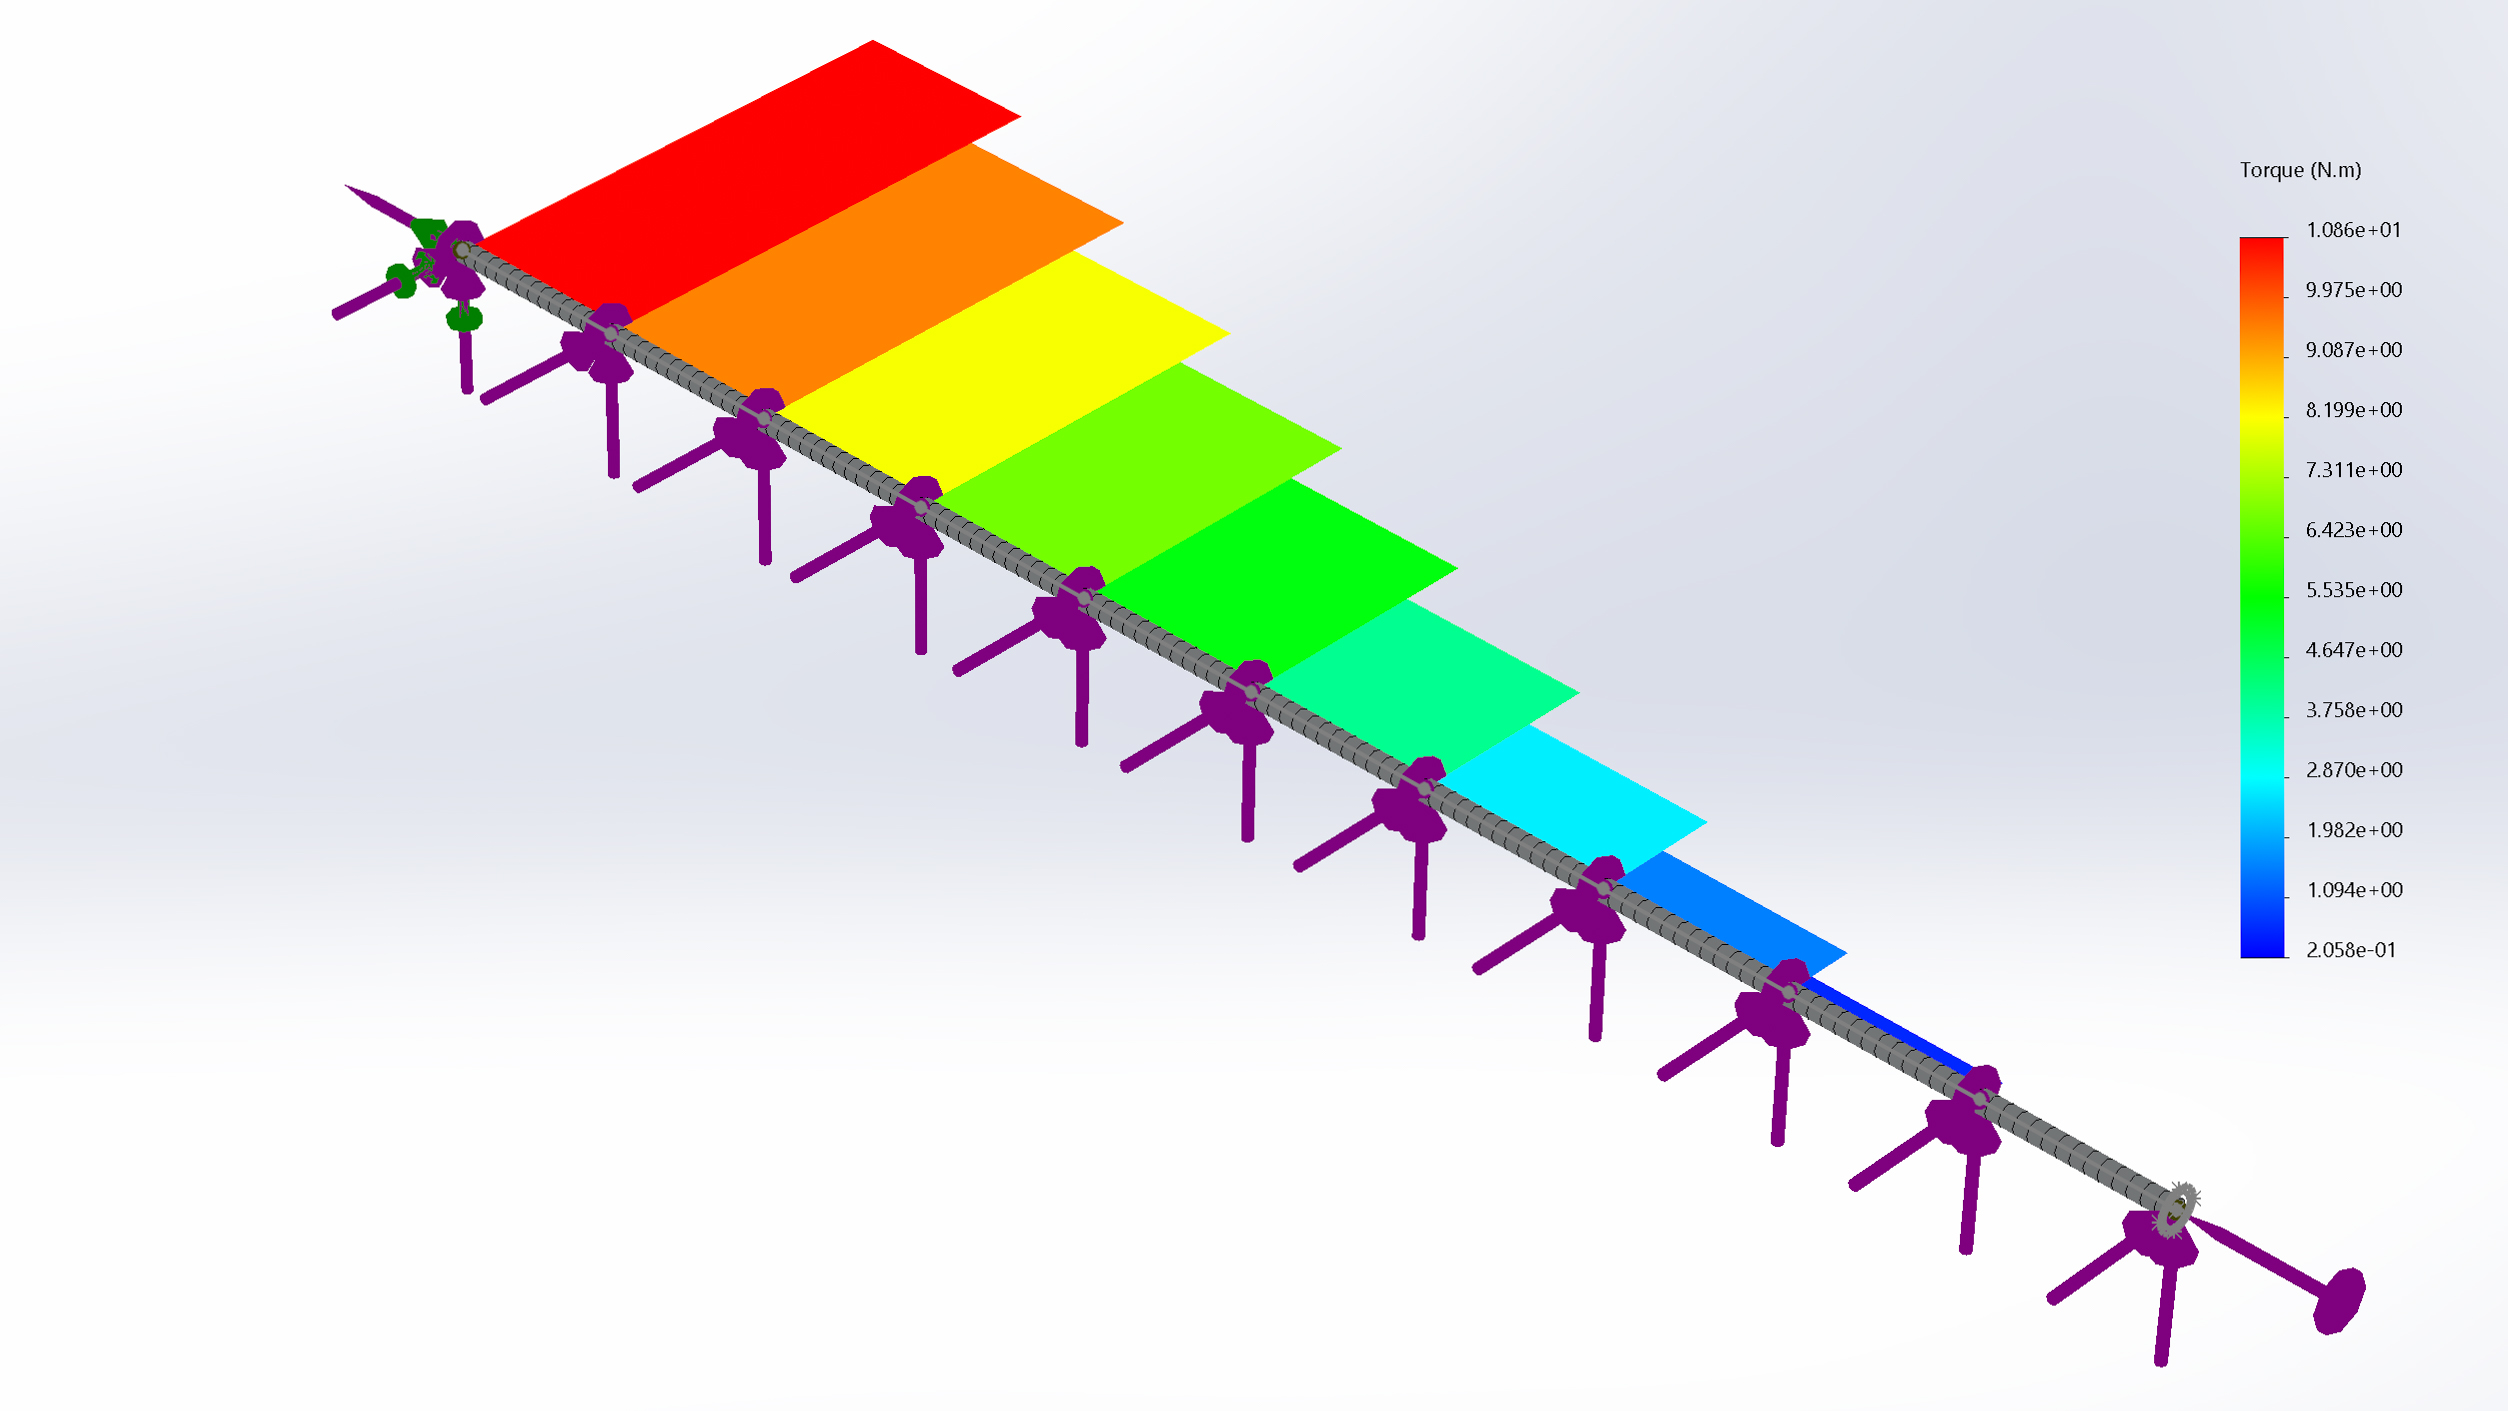
\includegraphics[width=\textwidth]{T.jpg}
      \caption*{Momento Torsor $T(y)$}
    \end{subfigure}
\end{figure}

\begin{figure}[H]
    \begin{subfigure}[b]{0.48\textwidth}
      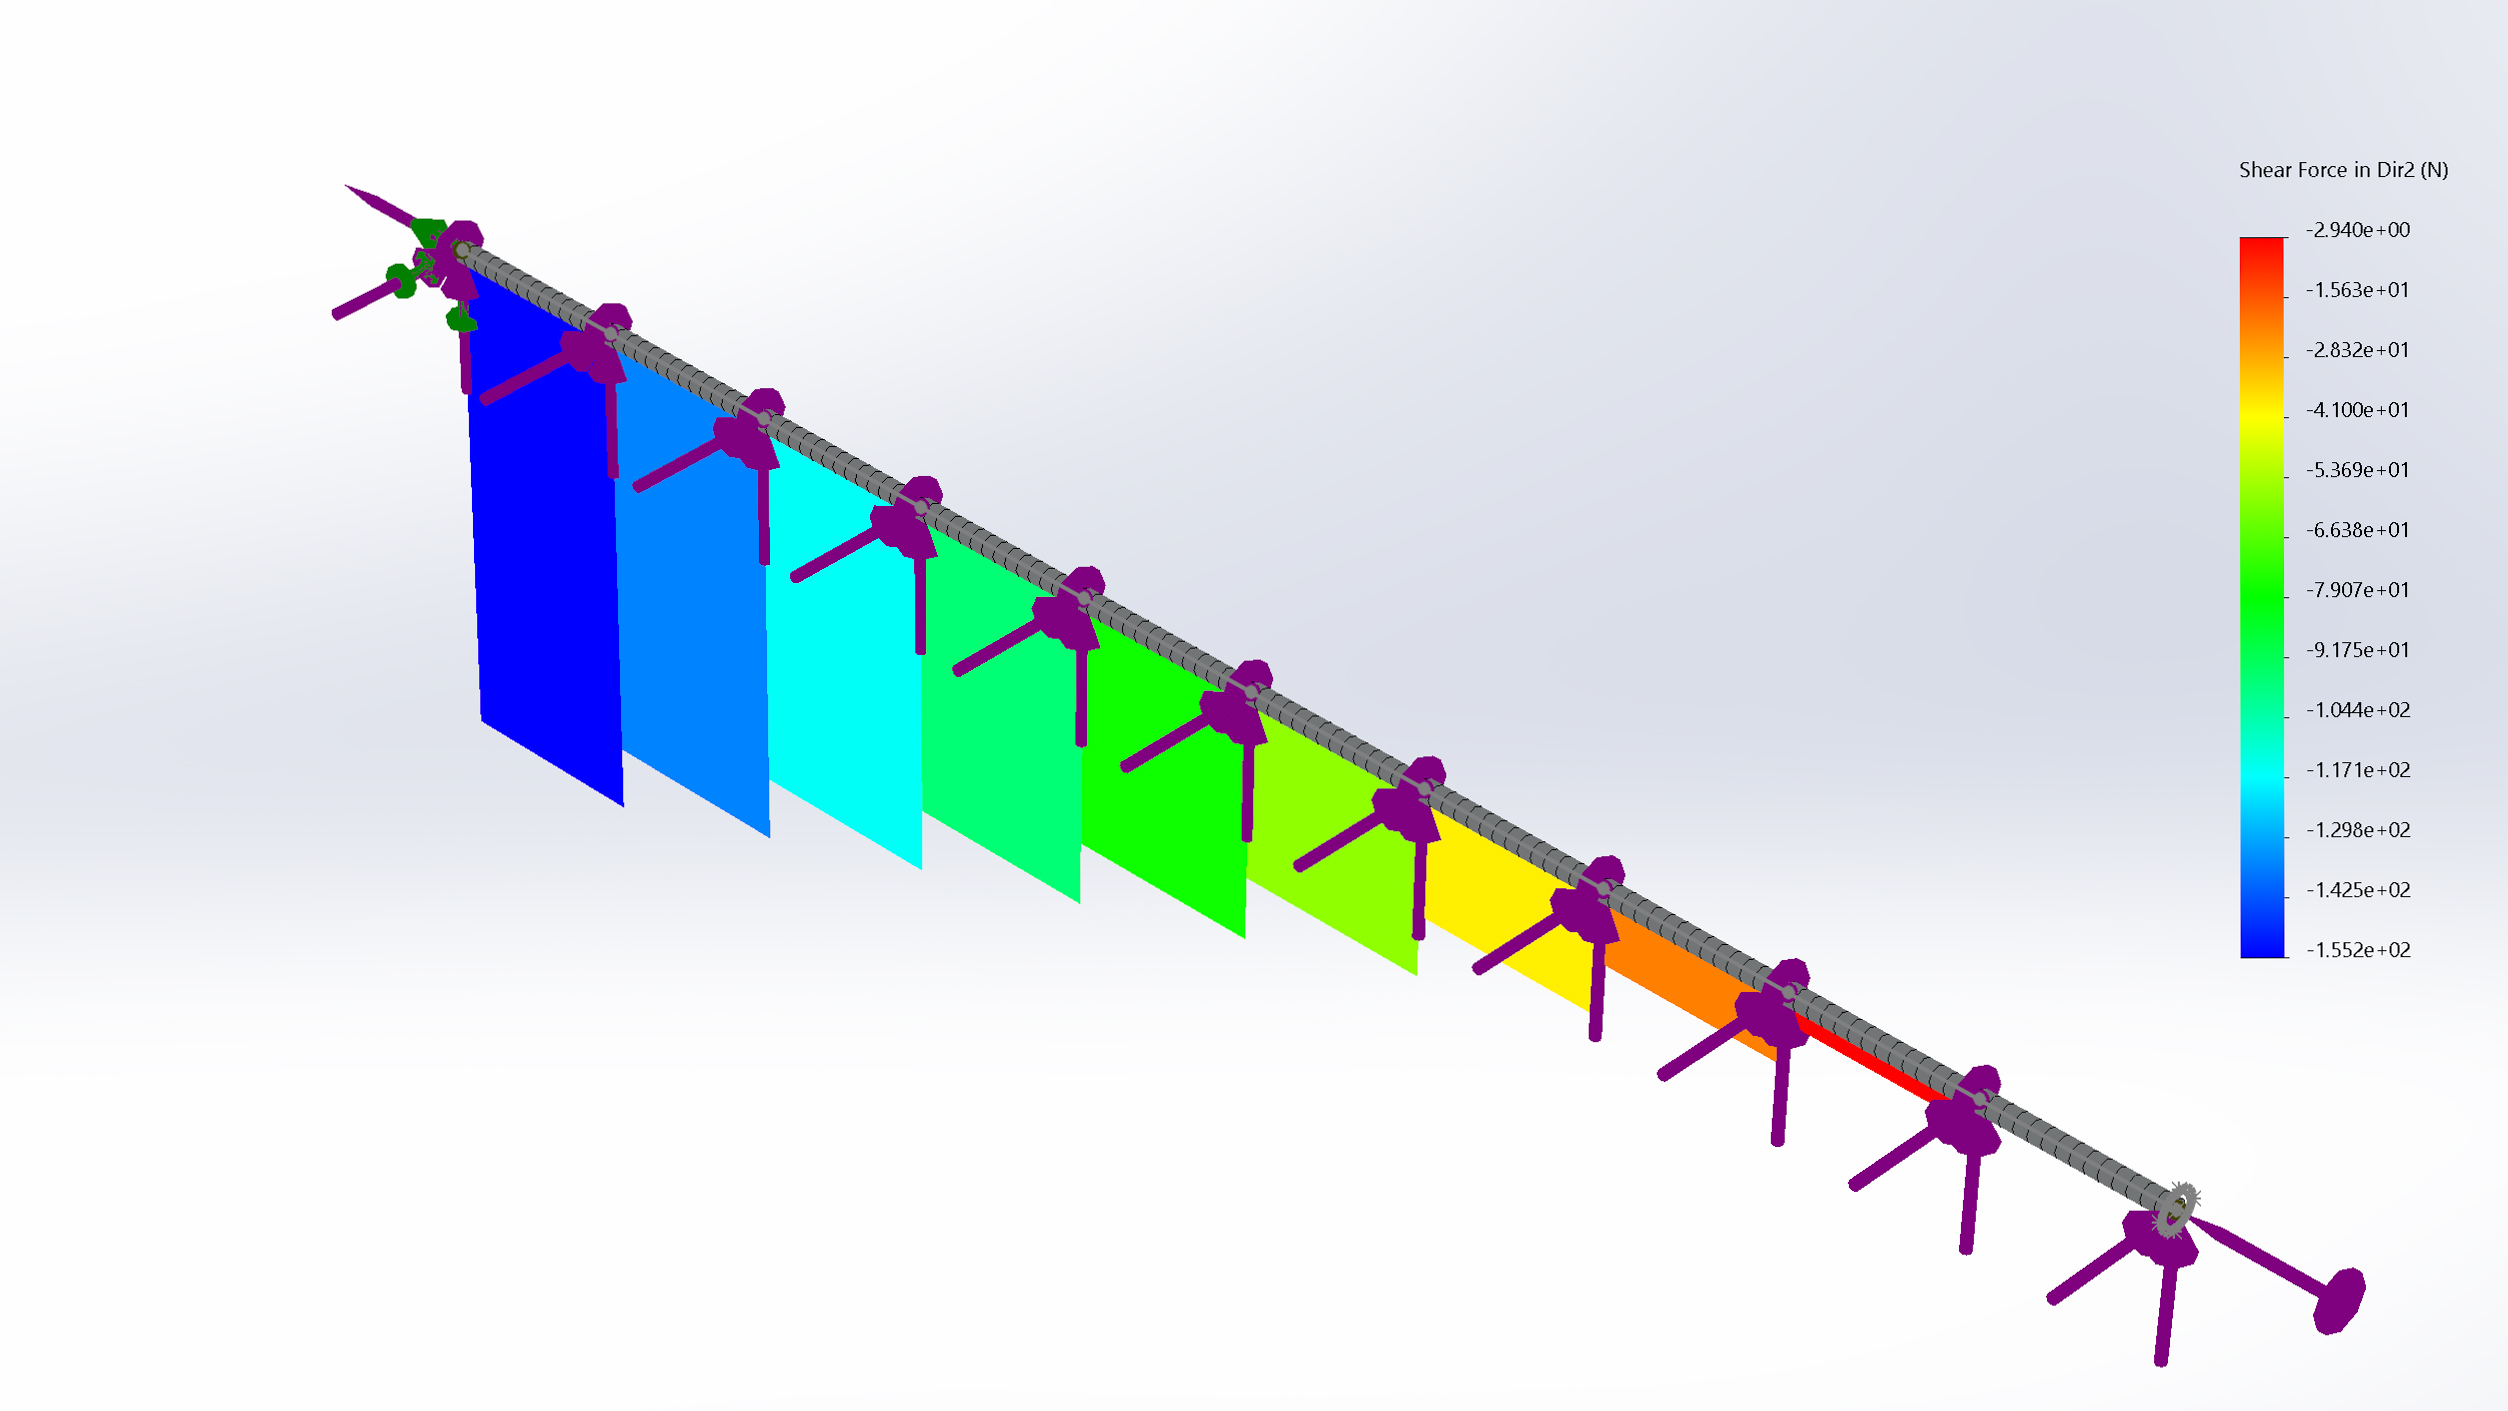
\includegraphics[width=\textwidth]{VL.jpg}
      \caption*{Força Cortante de L $V_z(y)$}
    \end{subfigure}
    %
    \begin{subfigure}[b]{0.48\textwidth}
      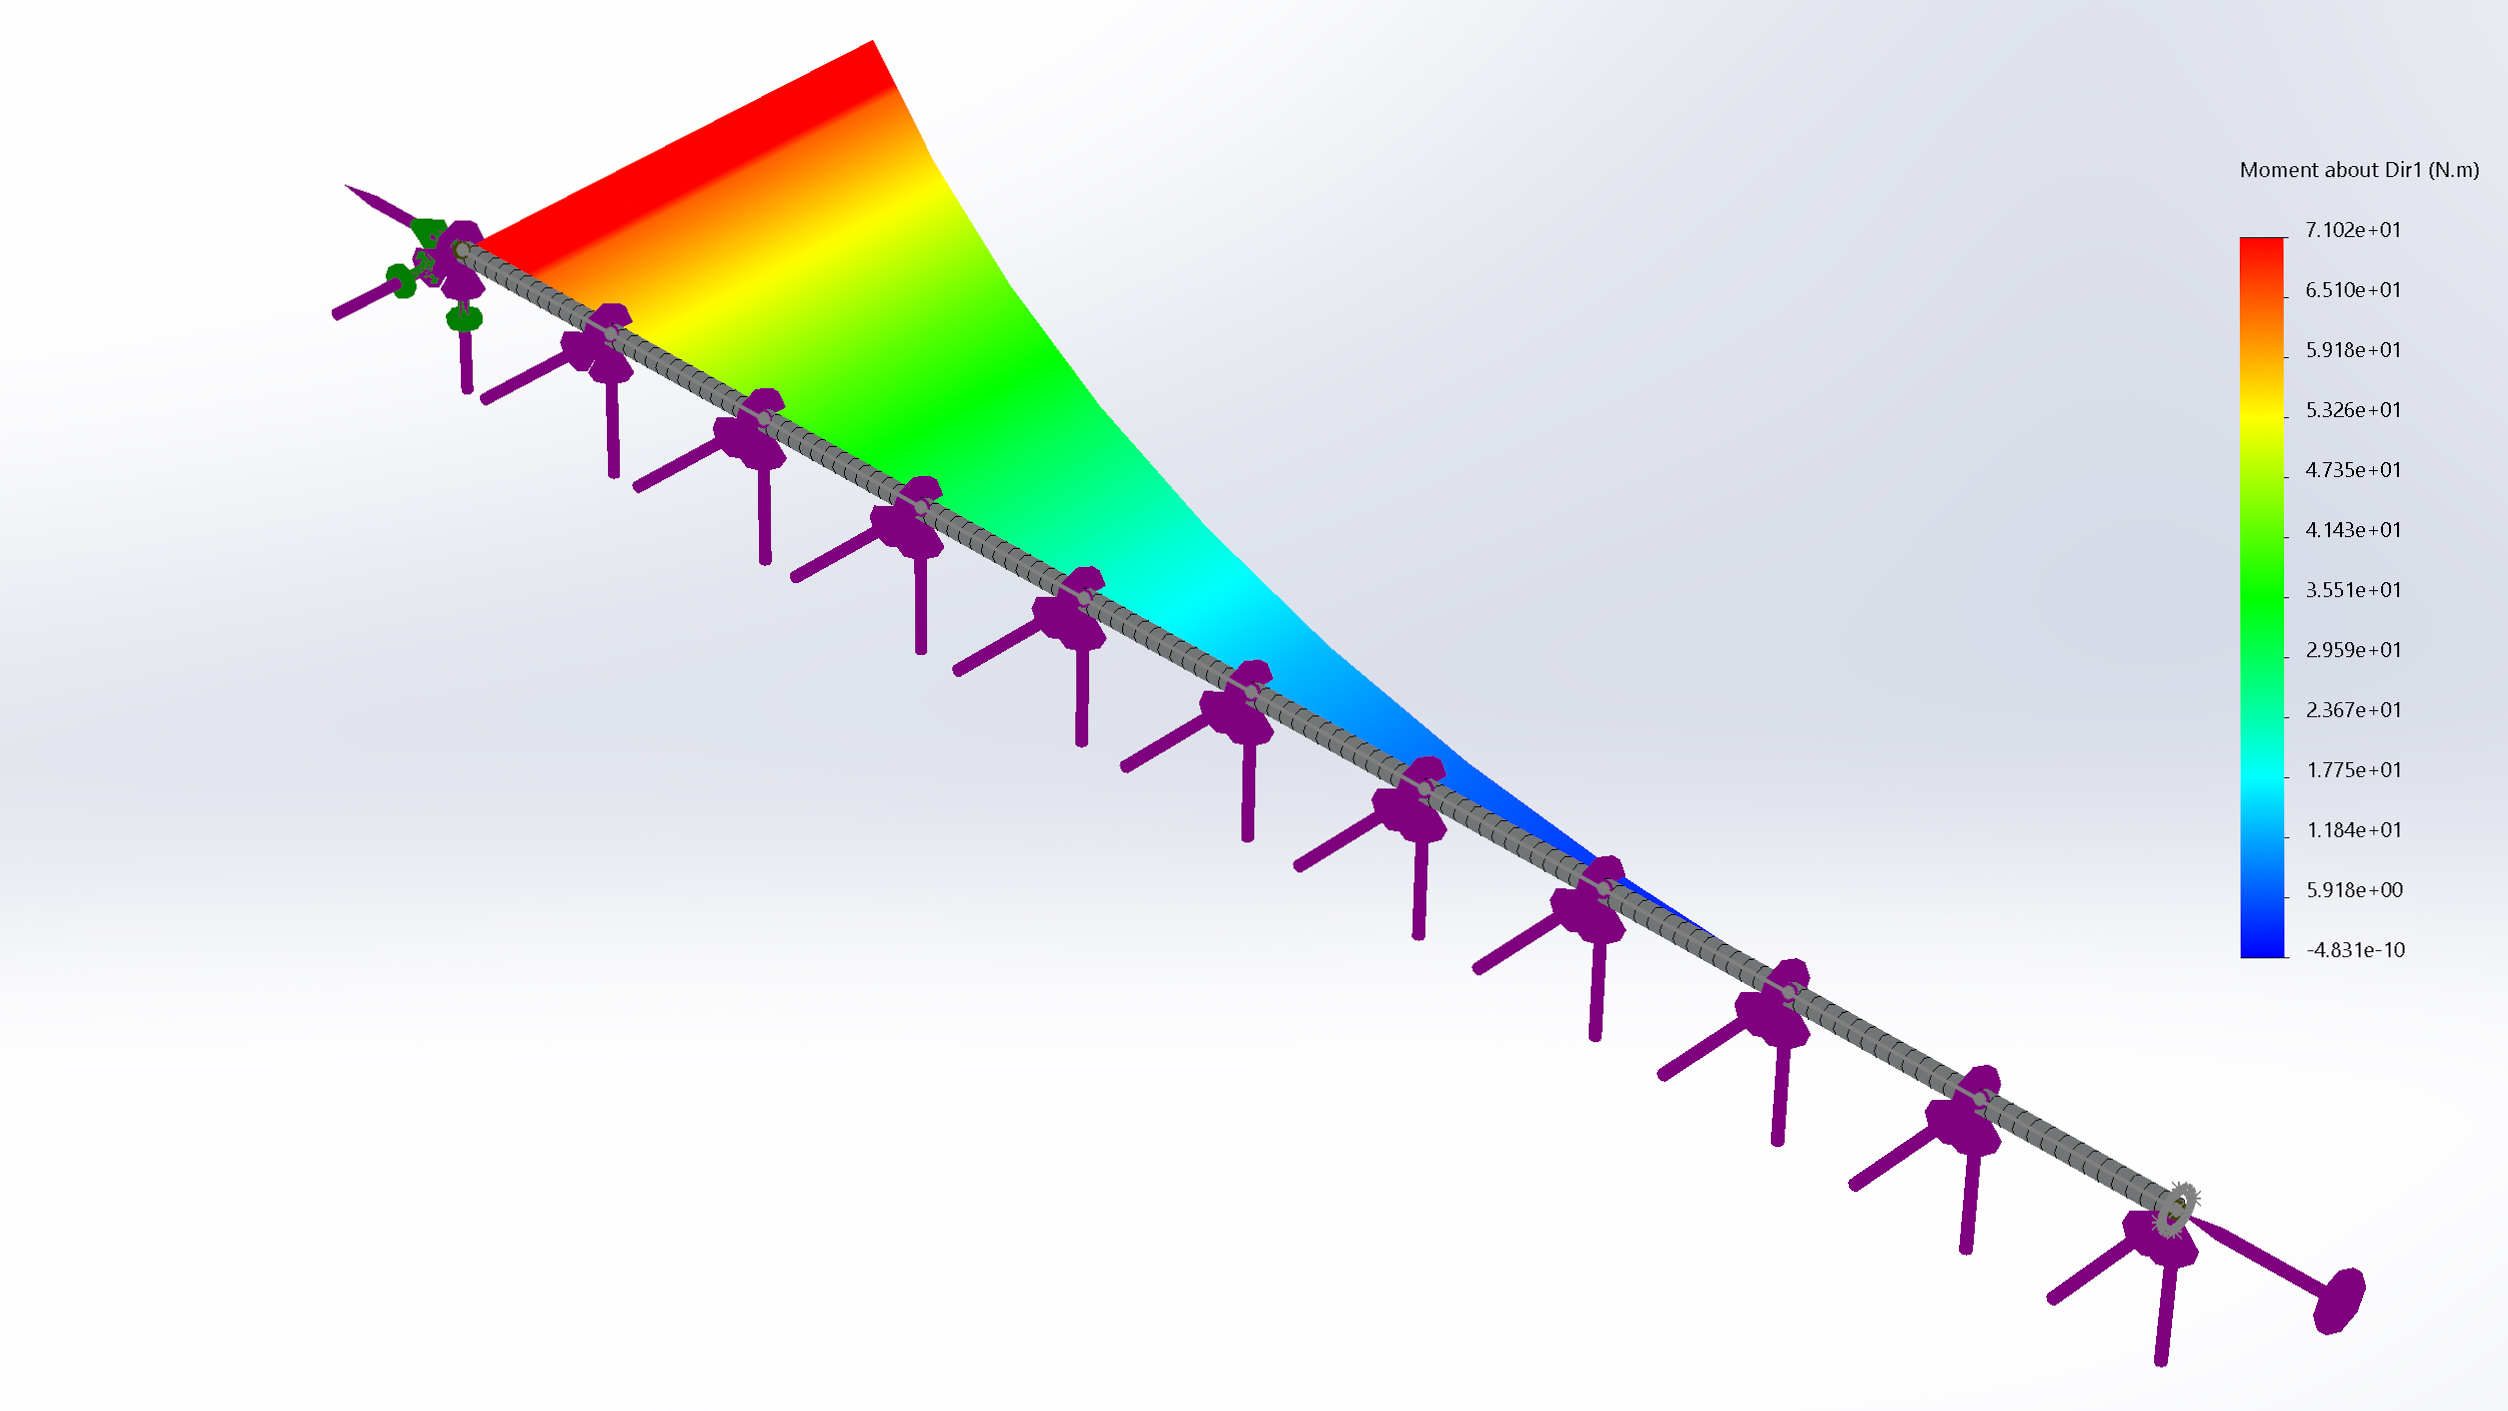
\includegraphics[width=\textwidth]{ML.jpg}
      \caption*{Momento de L $M_x(y)$}
    \end{subfigure}
\end{figure}

\begin{figure}[H]
    \begin{subfigure}[b]{0.48\textwidth}
      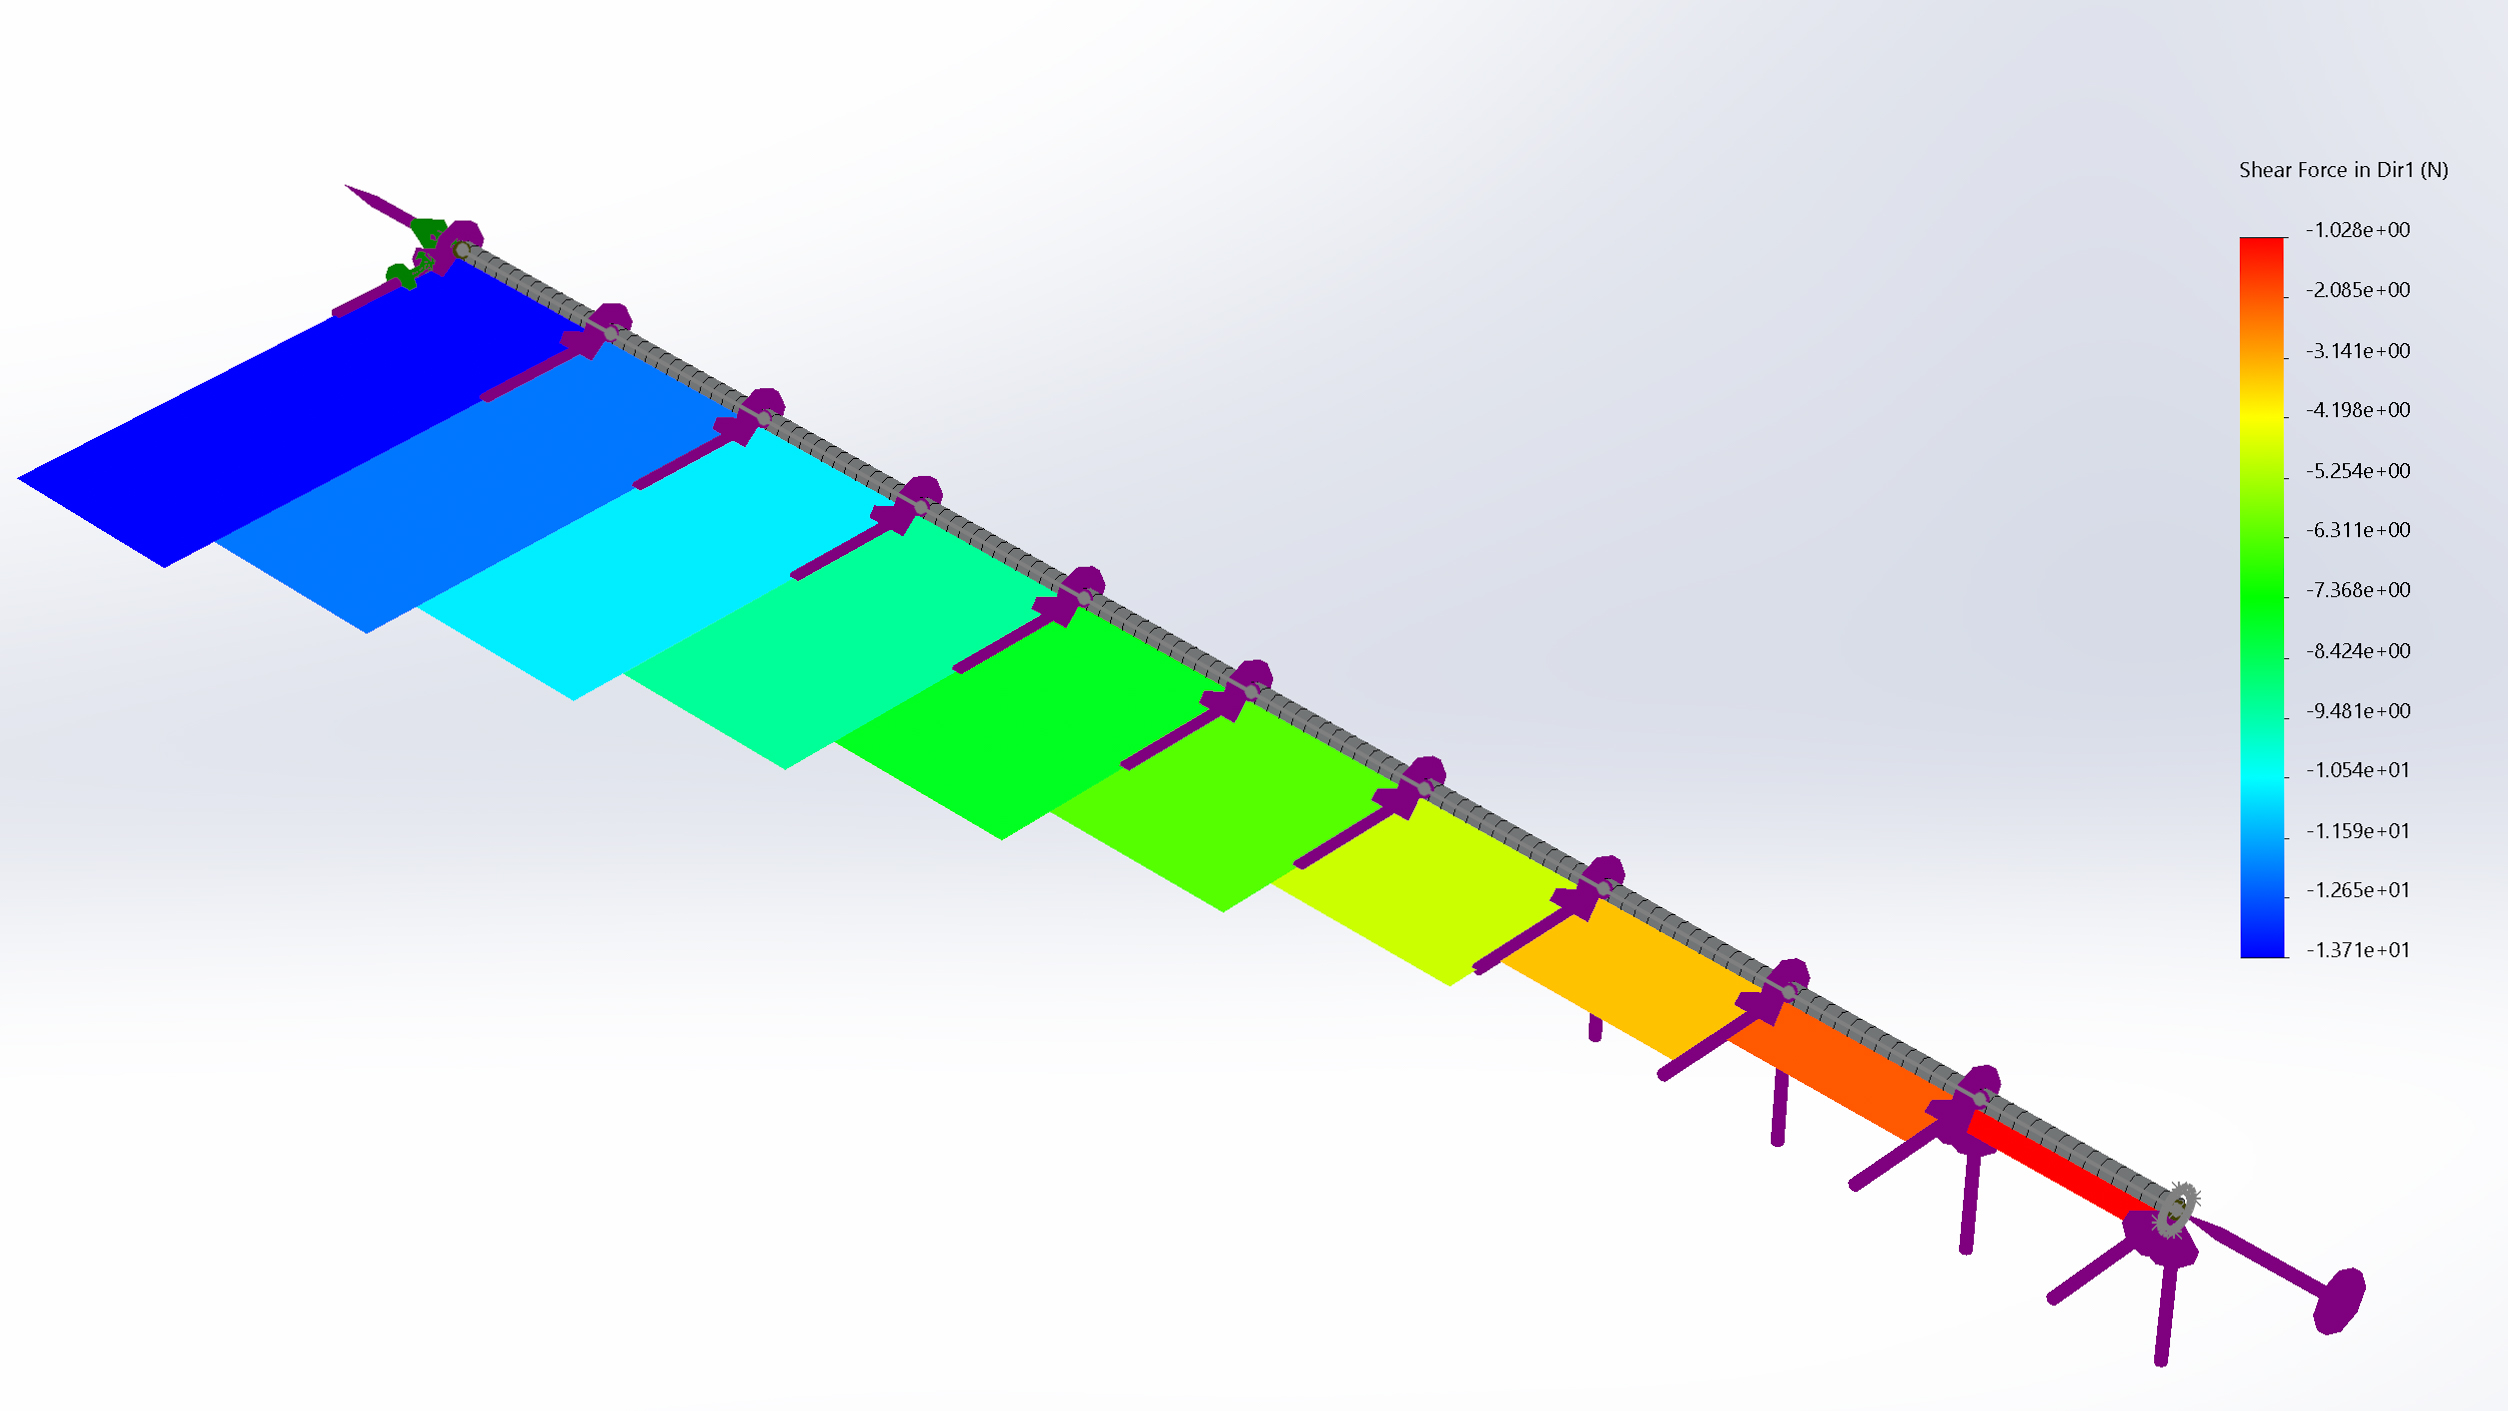
\includegraphics[width=\textwidth]{VD.jpg}
      \caption*{Força Cortante de D $V_x(y)$}
    \end{subfigure}
    %
    \begin{subfigure}[b]{0.48\textwidth}
      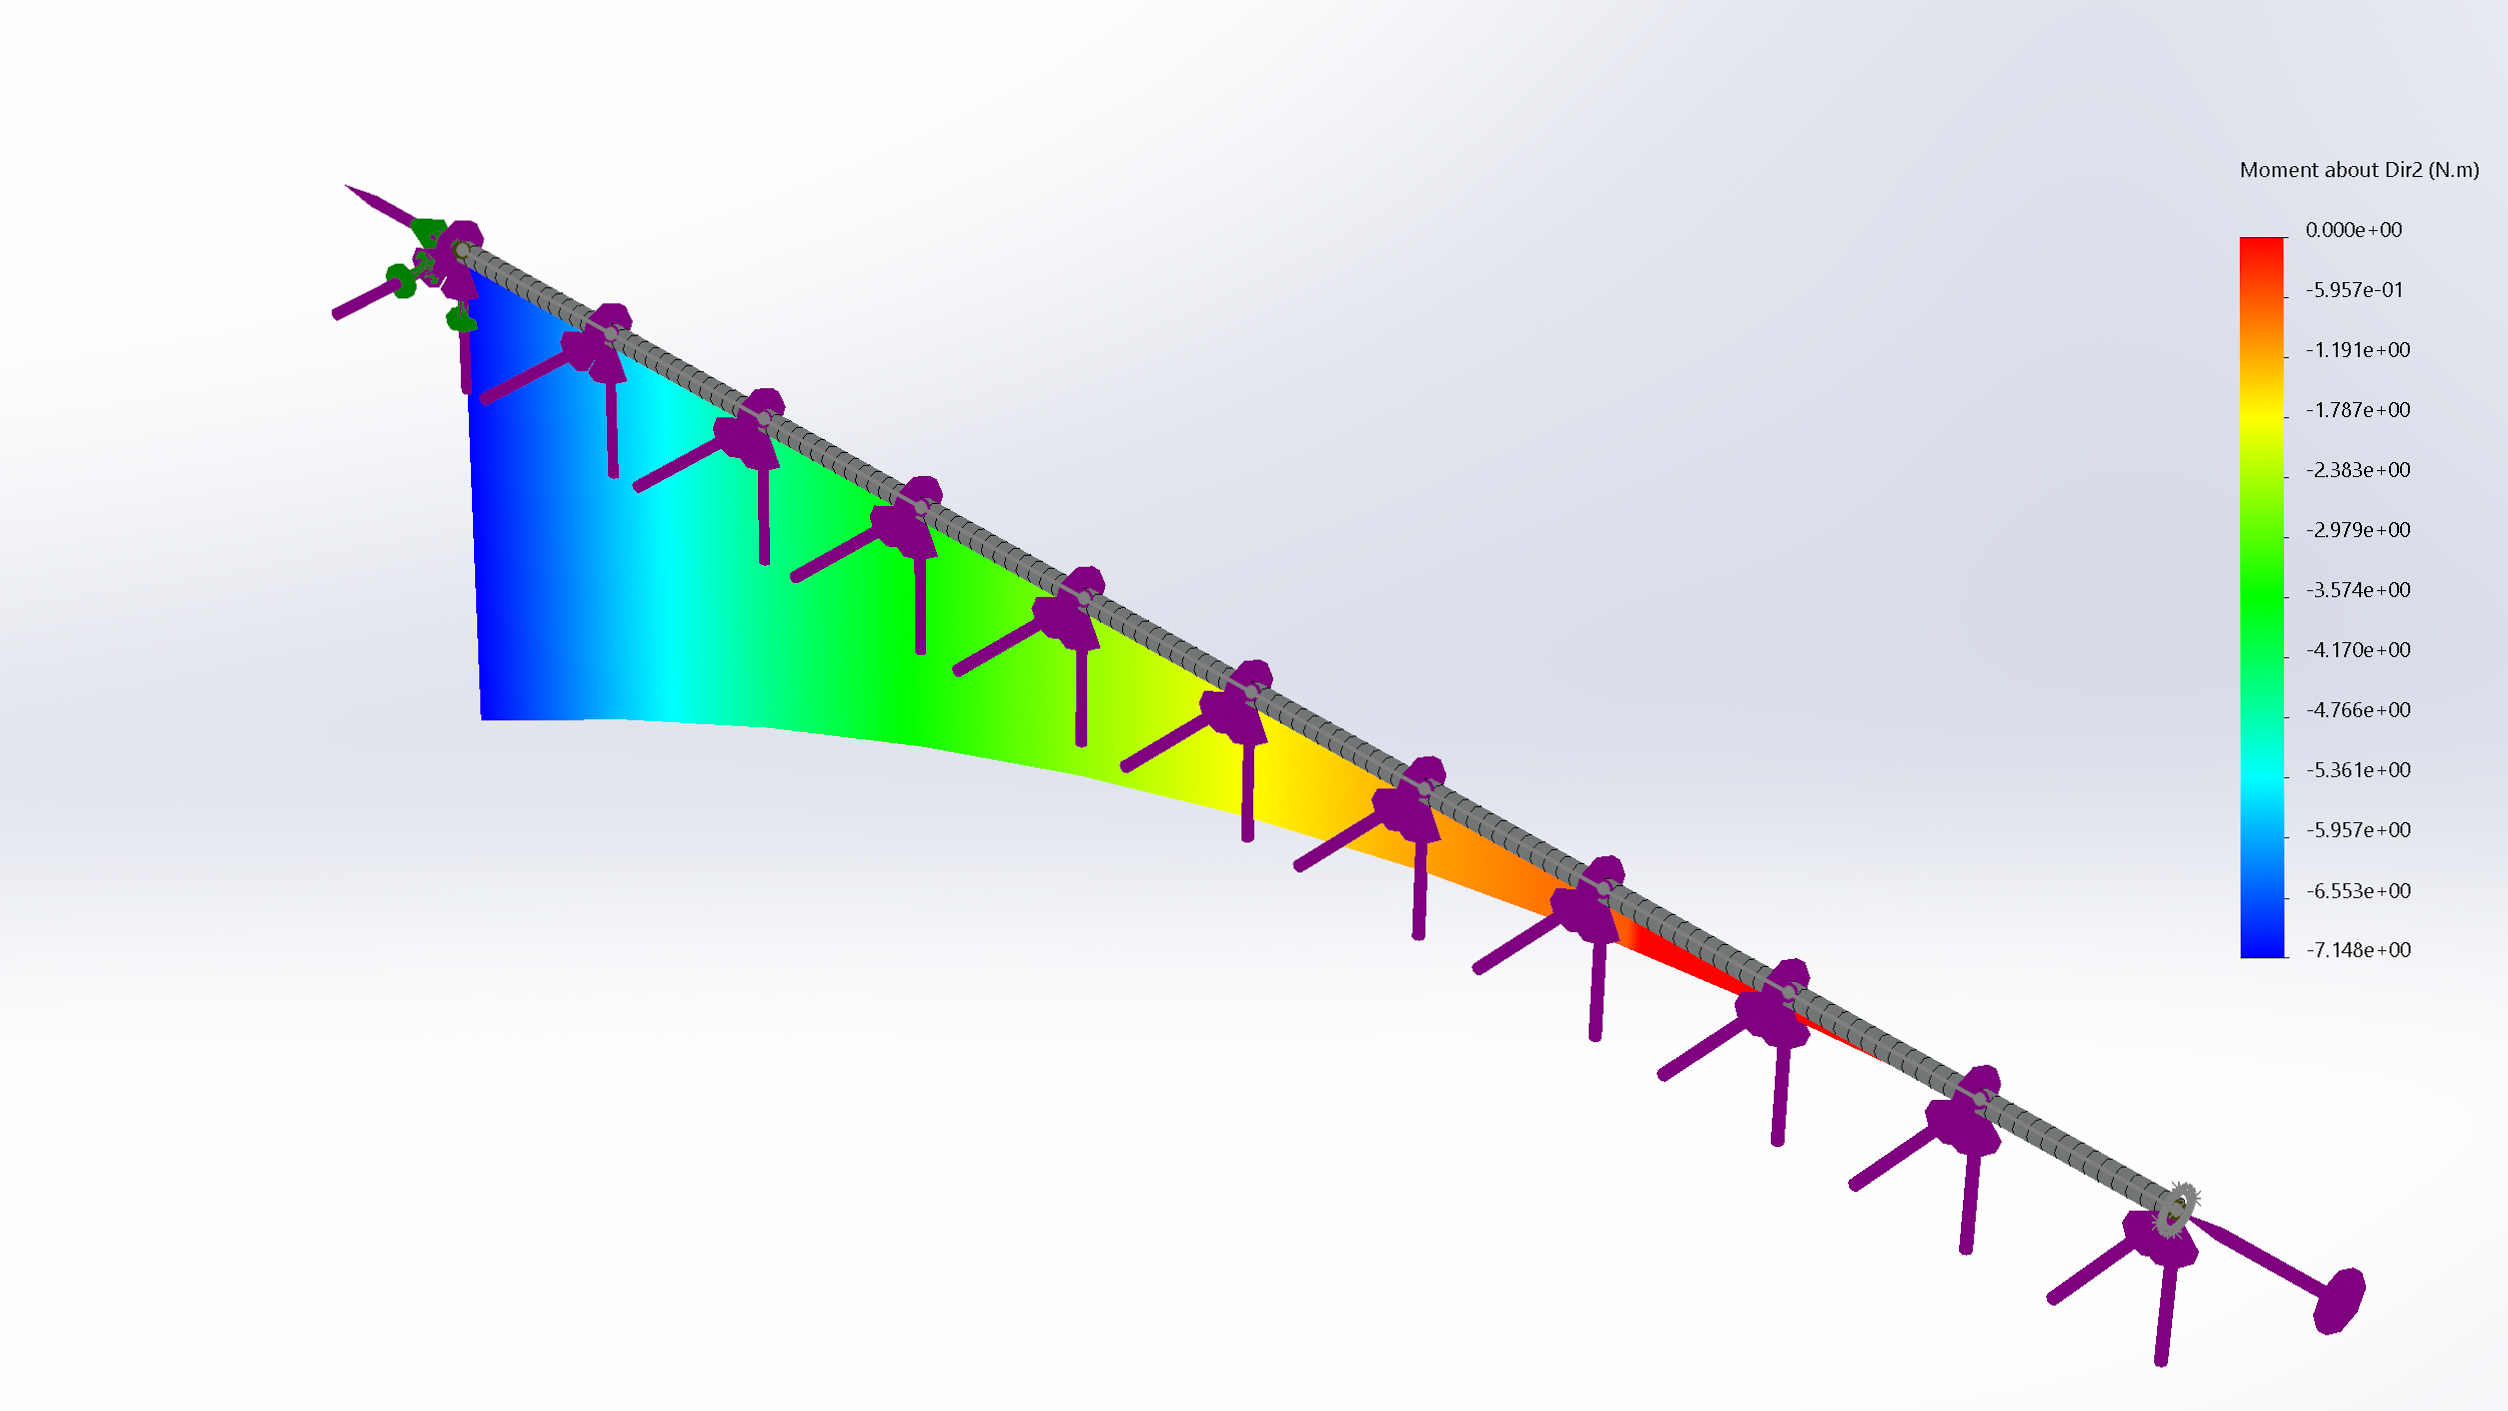
\includegraphics[width=\textwidth]{MD.jpg}
      \caption*{Momento de D $M_z(y)$}
    \end{subfigure}
\end{figure}

Conhecendo estas distribuições de força, podemos então analisar o efeito de materiais e seções retas distintas. Para este exemplo acima, a ferramenta disponibiliza apenas um tubo com diâmetro externo de 21.3 mm e 2.3 mm de espessura (padrão ISO), mas podemos transmitir estes resultados para seções também anulares com outras dimensões de diâmetro e espessura que mantenham aproximadamente a proporção entre a área de seção horizontal (a qual tem uma relação aproximadamente linear com as tensões internas para espessuras finas) e o momento de inercia desta seção. Uma das configurações que permite é justamente a apresentada abaixo.

\begin{figure}[H]
    \begin{subfigure}[b]{0.48\textwidth}
      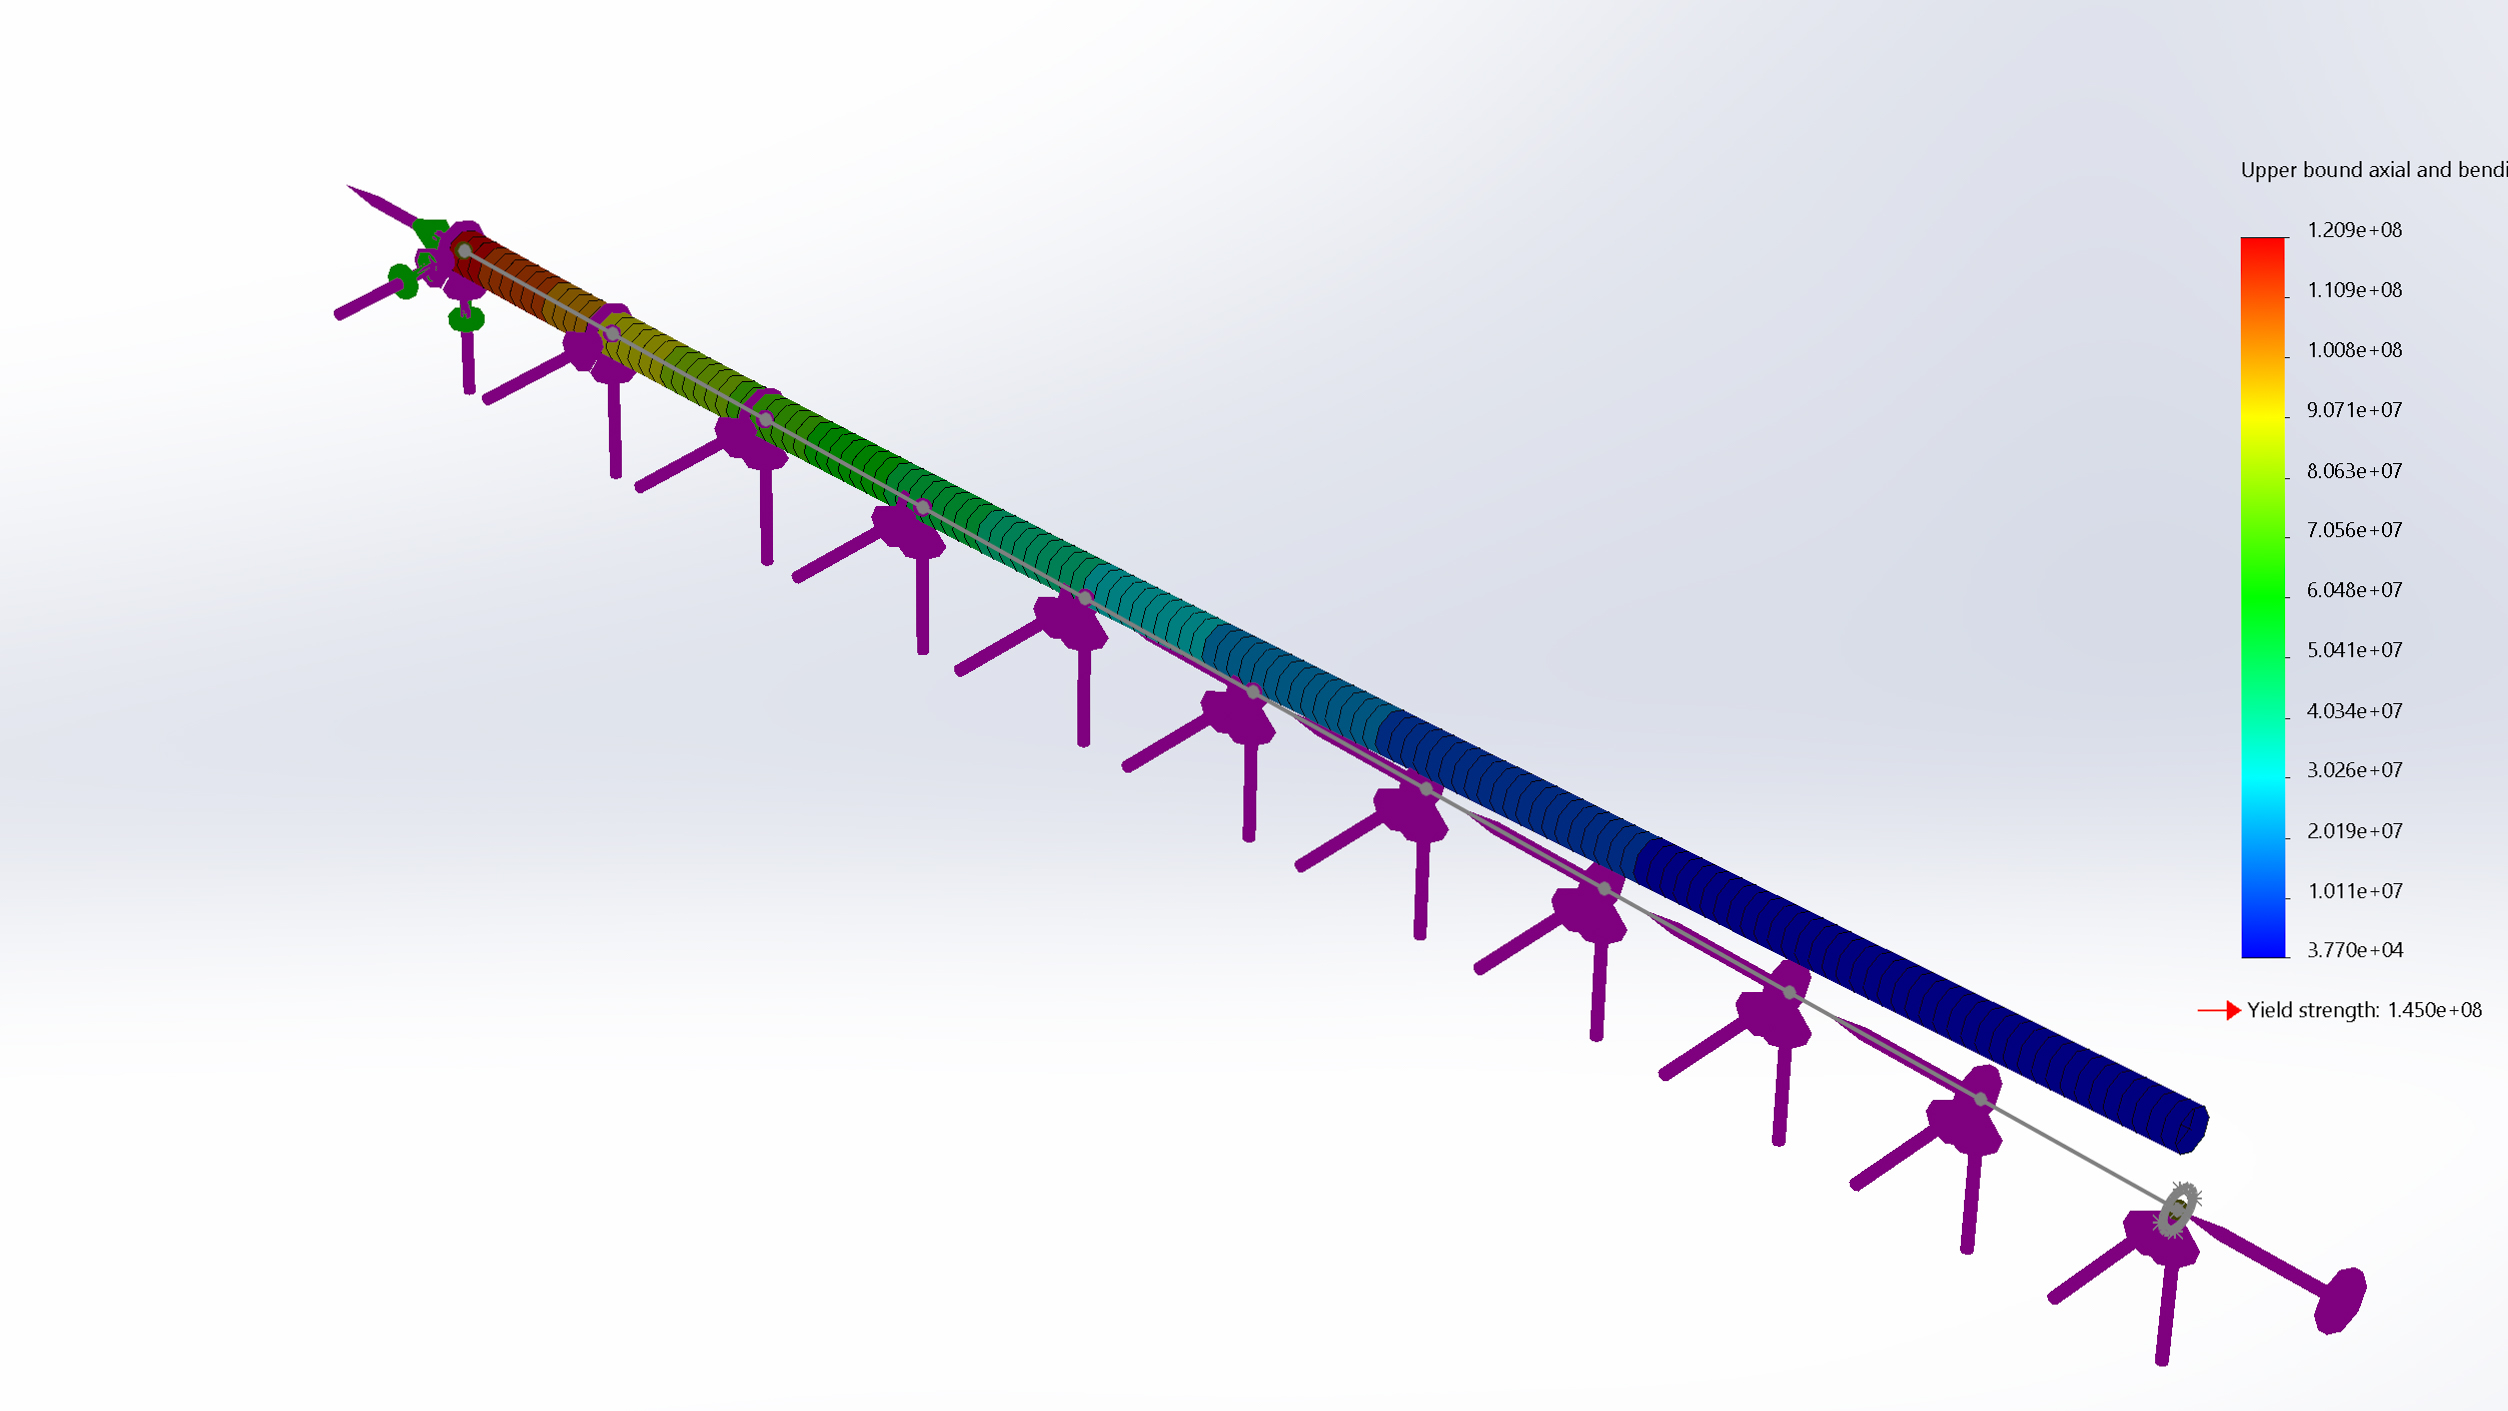
\includegraphics[width=\textwidth]{woMesh.jpg}
      \caption*{Barra com configurações limitadas}
    \end{subfigure}
    %
    \begin{subfigure}[b]{0.48\textwidth}
      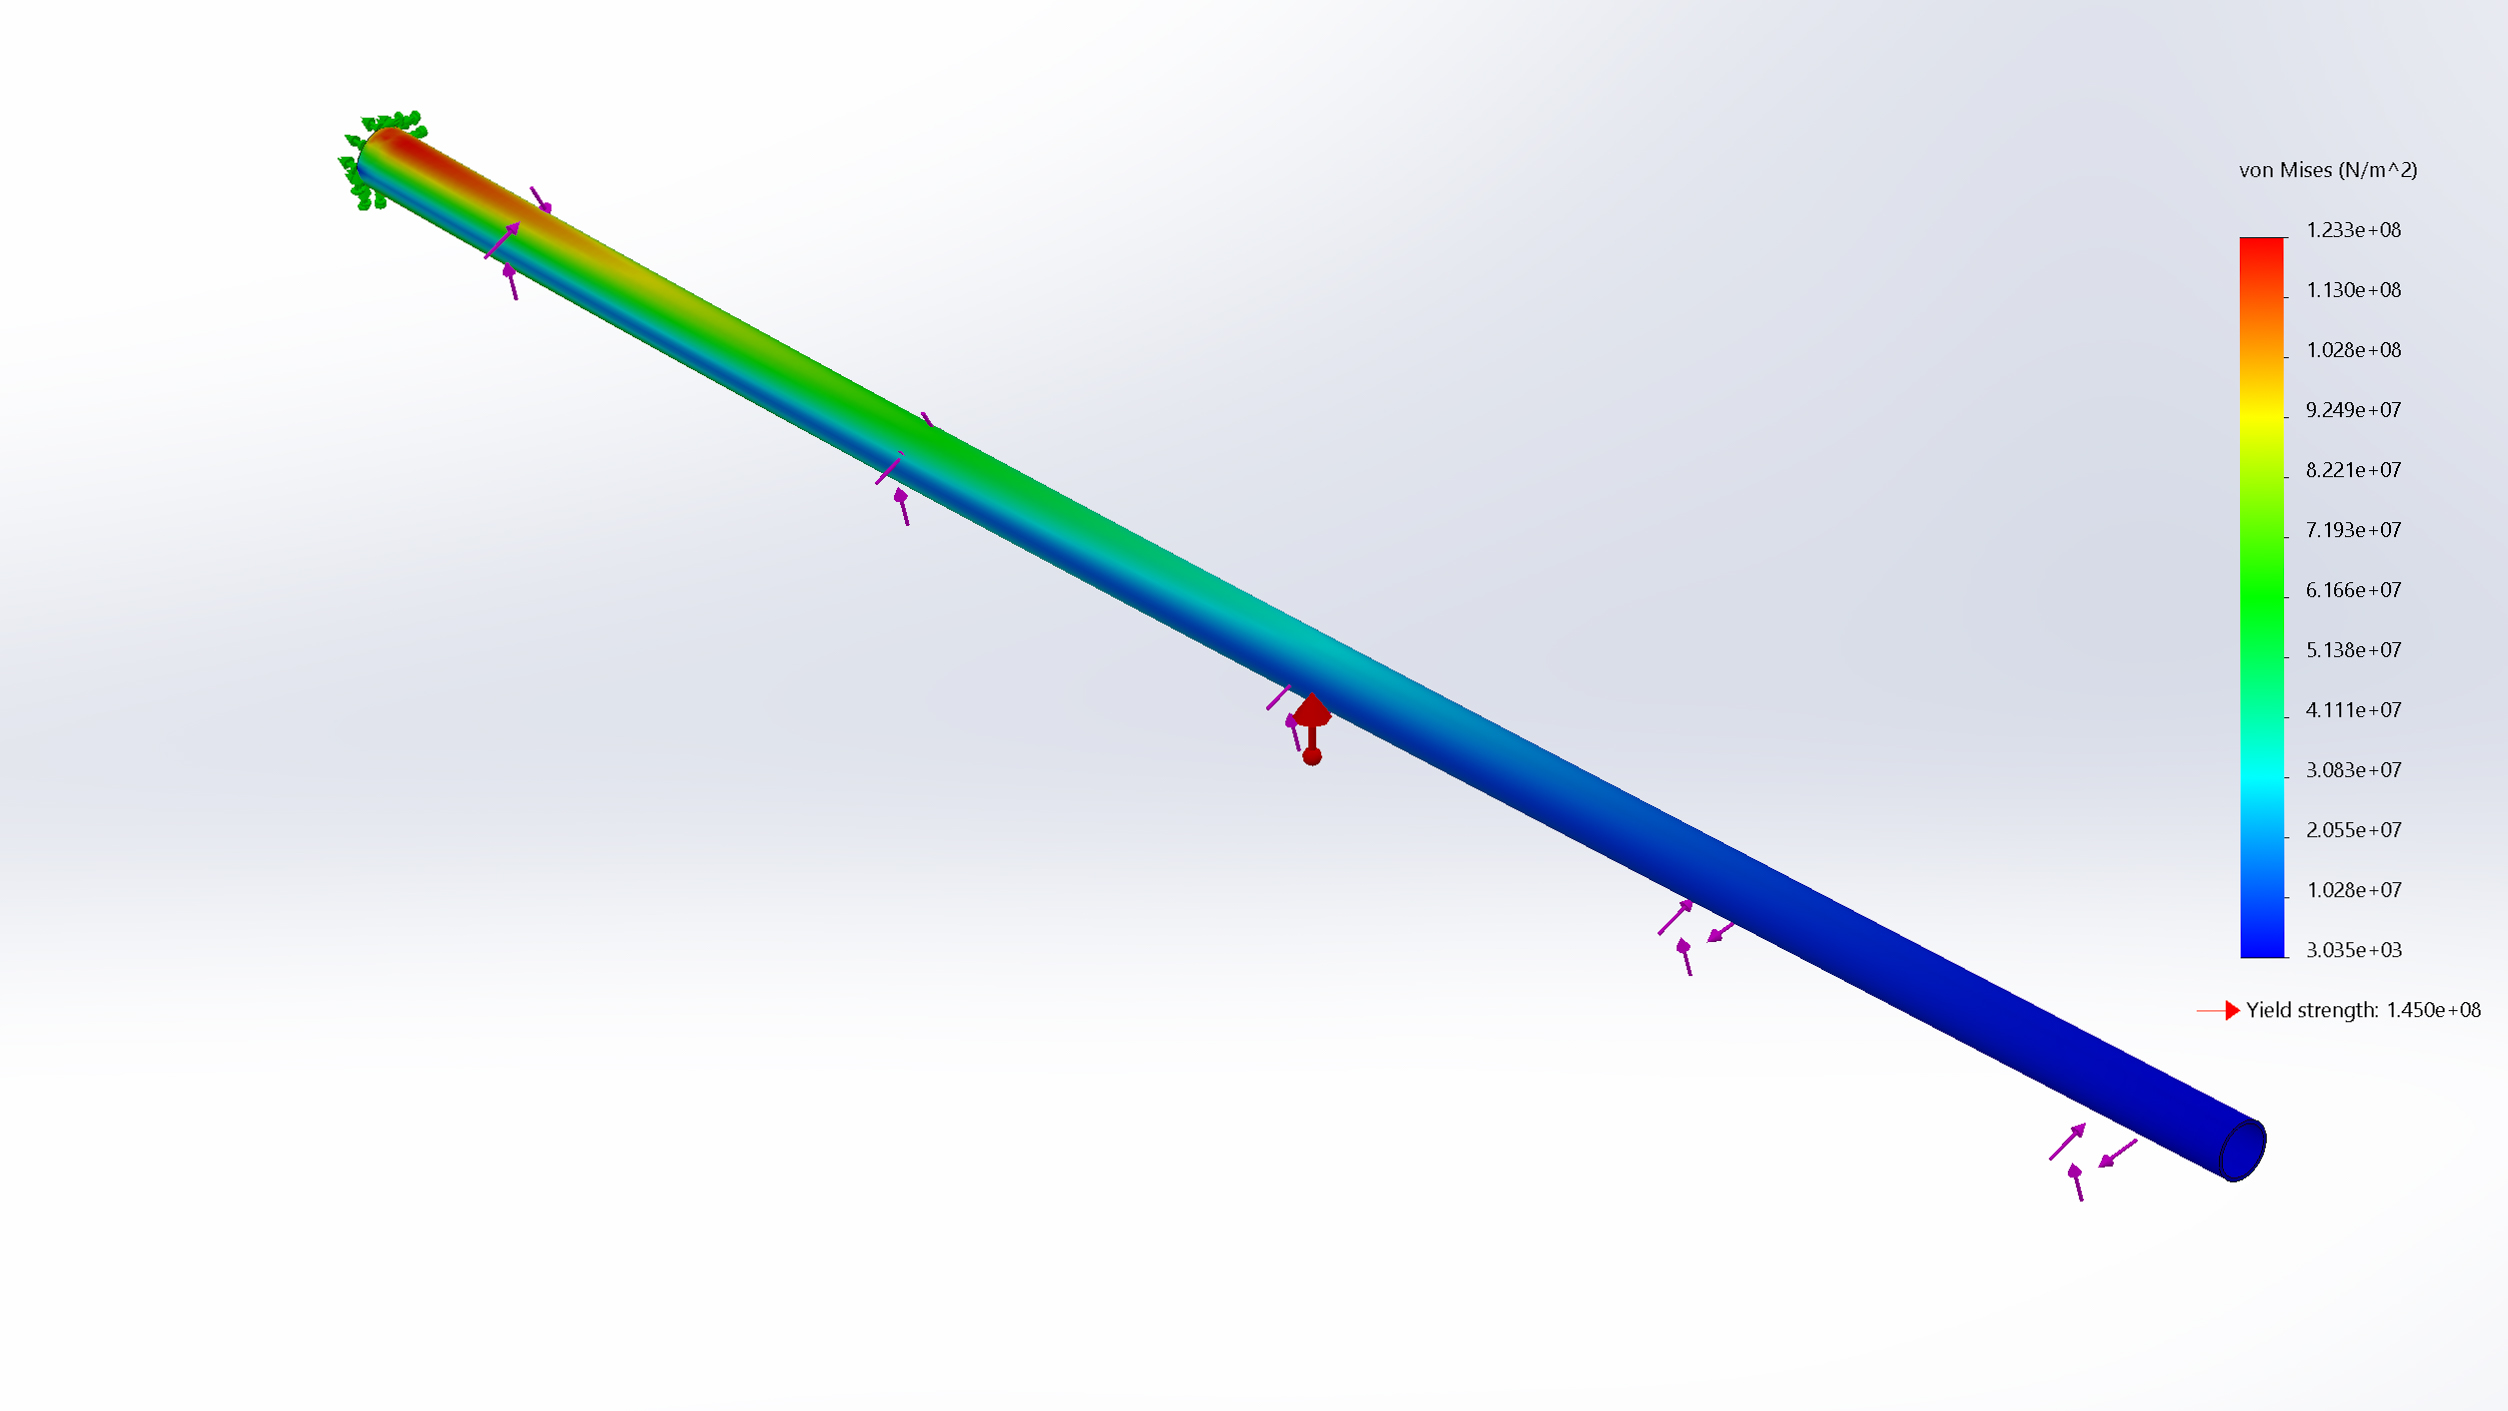
\includegraphics[width=\textwidth]{wMesh.jpg}
      \caption*{Barra comercial escolhida}
    \end{subfigure}
\end{figure}

A escolha do material é importante nos aspectos de deformação máxima da barra e tensão máxima de escoamento. Foram testados diversos materiais como PVC rígido, diferentes ligas de alumínio (especialmente da série 6000), e aço AISI 1020. A construção em PVC, além de ter uma deformação muito elevada para pequenas forças, ultrapassava seu limite de escoamento. O aço foi utilizado como referência e seria a escolha caso não fosse encontrada uma liga de alumínio que atendesse as especificações, mas sua densidade resultava em um peso final que exigiria a não-conformação com os requisitos estabelecidos. 

Para o alumínio, a melhor configuração que estava disponível no mercado foi um tubo de $25.4 mm$ ($1''$) com $1.58 mm$ de espessura de Alumínio estrudado 6063-T5, a qual atende a todos os requisitos com uma massa de $0.32 kg$ para a estrutura completa de uma asa. Além disso, considerando que o limite de escoamento desta liga é de $1.45 \times 10^8 N/m^2$, a estrutura nos dá um fator de segurança de aproximadamente $1.17$, o que é perfeito para uma aplicação aeronáutica não-tripulada, que deve ter uma performance elevada e seu custo de perda (especialmente em material e horas-trabalho) não é muito elevado.

\section{Correspondência aos Objetivos do Estudo}

Para entender a validade dos resultados obtidos, comparamos a seguir com os objetivos-pergunta da proposta do estudo aqui apresentado:

\begin{itemize}
    \item Considerando o tubo longitudinal que forma a longarina, o quão espeça deve ser parede do tubo considerando o carregamento esperado?
\end{itemize}

\noindent Com relação à proposta, foi feita a modificação de aumentar o diâmetro externo da longarina, motivado por uma mudança de configuração que permitiu diâmetros de $25.4mm$. Para este novo diâmetro, a espessura fica sendo igual a $1.58mm$ para alumínio 6063-T5 disponível em distribuidores como o seguinte: \url{https://www.aluminioalure.com.br/ye4hdjqia-tubo-redondo-de-aluminio-1-x-116-254cm-x-158mm}

\begin{itemize}
    \item Dados os possíveis materiais a serem utilizados na construção desta estrutura, quais os diâmetros de barras que seriam necessários para cada material?
\end{itemize}

\noindent Esta pergunta provou não ser muito pertinente para a análise dadas as limitações da ferramenta e/ou a não familiaridade com a mesma. É possível dizer que entre os 3 principais materiais considerados, o PVC exige dimensões incompatíveis com o aerofólio, o alumínio permite manter o diâmetro máximo e mesmo assim respeitar os limites de massa, o o aço pode ter um diâmetro ainda menor que o alumínio, mas não obedecia os requisitos de massa.

\begin{itemize}
    \item Em resultado da análise, é possível atingir todos os requisitos de design especificados com esta configuração de estrutura?
\end{itemize}

\noindent Sim. Todos os requisitos especificados na \textit{Proposta de Projeto} foram atingidos com êxito e mantendo uma margem considerável para utilização em estruturas associadas, como as nervuras, superfície aerodinâmica, e mesmo para os requisitos de primeira ordem sobre performance esperada.

\begin{thebibliography}{9}
    \bibitem{anacdrones} 
    Agência Nacional de Aviação Civil,   
    \textit{Orientações para Usuários de drones}.
    \\\url{www.anac.gov.br/assuntos/paginas-tematicas/drones/orientacoes\_para\_usuarios.pdf}

    \bibitem{xfoil} 
    Drela and Youngren,   
    \textit{XFOIL: Subsonic Airfoil Development System}.
    \\\url{https://web.mit.edu/drela/Public/web/xfoil/}

    \bibitem{aftools}    
    \textit{Airfoil Tools}.
    \\\url{http://www.airfoiltools.com/airfoil/details?airfoil=naca23015-il#polars}

    \bibitem{anderson}
    Anderson,
    \textit{Fundamentals of Aerodynamics, 6th ed}
    \\\texttt{ISBN 978-1-259-12991-9}

    \bibitem{WPIpaper}
    Sathaye,
    \textit{Lift Distributions on Low Aspect Ratio Wings at Low Reynolds Numbers},
    \\M.Sc. Thesis, Worcester Polytechnic Institute

\end{thebibliography}

\end{document}